\chapter{线性空间、映射与坐标}
\label{chap:linear-representation}
\label{chap:linear-algebra-and-matrix-analysis}
\label{chap:linear-algebra}

第~\ref{chap:linear-operations}章把数据记成数组，并规定了数组的运算，但没有区分数组本身和它记录的对象。以仿射函数$f_{a,b}(t)=a+bt$为例。它是一个函数，两个仿射函数相加或缩放后仍是仿射函数。选定$1$与$t$这两个基本函数以后，$f_{a,b}$才记成一列数$(a,b)^{\top}$；换一组基本函数，这列数随之改变，函数本身却不变。

矩阵同样有两重身份。设计矩阵$\bm X_\varepsilon$（式~\eqref{eq:linear-algebra-nearly-collinear-design}）是一张$3\times2$的数表，它还记录了一个作用：把两个系数送到三个拟合值。要在不同的记录之间换算，又不被记录方式误导，就要把对象和记录对象的数分开。

本章按这一区分展开。记录之前，先要说清对象在什么范围内作线性组合：第~\ref{sec:ls-vector-spaces}节把数组、函数等能相加和缩放的对象统一为线性空间，并研究其中对线性组合封闭的子空间，以及“有意忽略一个子空间中的差别”得到的商空间。第~\ref{sec:ls-bases-dimension-coordinates}节在空间中选定一组基，用张成与线性无关保证每个对象有唯一的一组系数，即坐标；基的个数给出维数，换基时坐标按可逆矩阵换算，对象本身不变。

对象记录清楚以后，再记录对象之间保持线性组合的作用。第~\ref{sec:ls-linear-maps}节说明，选定两端的基，线性映射就记成矩阵；核与像分别描述映射消去的输入和能到达的输出；换基改变矩阵而不改变映射，由此得到相抵与相似两种关系。把向量线性地读成一个数的规则，即线性泛函，留到第~\ref{chap:dual-spaces}章。

本章在实数域上展开，涉及复数时另作说明。全章只用加法和数乘，所需的矩阵运算都来自第~\ref{chap:linear-operations}章；长度与收敛由第~\ref{chap:normed-spaces}章引入，夹角与正交由第~\ref{chap:inner-product-spaces}章引入。

% 第2章第1节：线性空间与子空间（向量空间；子空间及其包含、交、和、直和与商空间）。

\section{线性空间与子空间}
\label{sec:ls-vector-spaces}
\label{sec:linear-algebra-vector-spaces-coordinates}

第~\ref{chap:linear-operations}章的数组和本章开头的仿射函数都能相加和缩放。用一组方向记录这些对象之前，要先说清线性组合在什么范围内进行。本节先给出线性空间的定义，再讨论空间内部对线性组合封闭的部分，即子空间，以及子空间之间的比较、合并和商空间。

\subsection{线性空间的定义与示例}
\label{sec:ls-space-axioms}

第~\ref{sec:ls-vector-operation-rules}节验证过，同形数组的加法与数乘满足八条运算规则。其他对象也满足同样的规则：平面上的位移可以首尾相接，有限信号可以按幅度放大，多项式可以逐点相加。后面关于分解、方程的解和维数的结论只用到这八条规则，与对象具体是数组、位移、信号还是多项式无关。

因此，把带有这样的加法与数乘的集合统称为线性空间，其中的元素统称为向量。从此，“向量”指可以作线性组合的对象，不再要求它是一列数。

\begin{definition}[实线性空间]
\label{def:ls-real-vector-space}
设$V$是一个集合，给定加法（任意$\bm u,\bm v\in V$对应$\bm u+\bm v\in V$）与实数数乘（任意$a\in\mathbb R$、$\bm u\in V$对应$a\bm u\in V$）。若对任意$\bm u,\bm v,\bm w\in V$和$a,b\in\mathbb R$，下面八条规则成立，就称$V$为\term{向量空间}（也称线性空间，vector space）：
\begin{enumerate}
 \item 加法交换律：$\bm u+\bm v=\bm v+\bm u$。
 \item 加法结合律：$(\bm u+\bm v)+\bm w=\bm u+(\bm v+\bm w)$。
 \item 零元：存在$\bm0\in V$，使$\bm u+\bm0=\bm u$对每个$\bm u$成立。
 \item 加法逆元：每个$\bm u$都有$-\bm u\in V$，使$\bm u+(-\bm u)=\bm0$。
 \item 数乘结合律：$a(b\bm u)=(ab)\bm u$。
 \item 数乘对数的分配律：$(a+b)\bm u=a\bm u+b\bm u$。
 \item 数乘对向量的分配律：$a(\bm u+\bm v)=a\bm u+a\bm v$。
 \item 单位数乘：$1\bm u=\bm u$。
\end{enumerate}
\end{definition}
定义包含两层要求。第一层是\emph{封闭}：加法和数乘的结果必须留在$V$中，否则运算无法在$V$内进行。第二层是\emph{规则}：前四条说加法像数的加法一样可以交换、结合，有零元和相反元；后四条说数乘与加法按熟悉的方式配合。

有了这些规则，有限次线性运算无论怎样加括号、怎样展开，结果都相同。所以对任意$\bm v_1,\ldots,\bm v_k\in V$与实数$a_1,\ldots,a_k$，加权和$\sum_{j=1}^ka_j\bm v_j$有确定的意义。它仍称为这组向量的线性组合，与第~\ref{sec:ls-vector-operations}节对数组的定义一致。

标量也可以取复数。复线性空间满足同样的八条规则，只是数乘允许任意复数。

允许哪些标量会改变线性结构。$\mathbb C$作为复线性空间时，每个元素都是$1$的复数倍；只允许实数数乘时，表示$a+b\mathrm i$需要$1$与$\mathrm i$两个方向。复数域上的基与线性映射按同样的方式定义，内积则要处理共轭。本章其余推导在实数域中进行。

常见的具体空间都满足定义。$\mathbb R^d$与全体$m\times d$实矩阵在逐项运算下是线性空间，第~\ref{sec:ls-vector-operation-rules}节已逐条验证。次数不超过$k$的实多项式组成的集合
\[
 P_k=\{a_0+a_1t+\cdots+a_kt^k:a_0,\ldots,a_k\in\mathbb R\}
\]
在逐点相加与数乘下也是线性空间：两个这样的多项式相加或乘以实数，次数仍不超过$k$；八条规则则逐点继承实数运算的规则。本章开头的仿射函数全体正是$P_1$。

并非每个由向量组成的集合都是线性空间。下面两个$\mathbb R^d$的子集沿用$\mathbb R^d$的运算，分别破坏了加法封闭与数乘封闭。
\begin{example}[反例：仿射约束集与非负向量集]
\label{ex:ls-non-vector-space-sets}
考虑第一坐标固定为$1$的向量与各坐标都非负的向量：
\[
 \begin{gathered}
S_1=\{\bm x\in\mathbb R^d:x_1=1\}\\
S_2=\{\bm x\in\mathbb R^d:x_j\geq0,\ j=1,\ldots,d\},
 \end{gathered}
\]
两者都沿用$\mathbb R^d$的逐项加法与数乘。

$S_1$的问题出在加法上。任取$\bm x,\bm y\in S_1$，和的第一坐标是
\[
 x_1+y_1=2\neq1,
\]
所以$\bm x+\bm y$已经离开$S_1$；同样，零向量的第一坐标为$0$，$S_1$连零向量都不含。

$S_2$则相反：两个非负向量相加仍然非负，加法没有问题，但数乘允许负数。$\bm e_1$属于$S_2$，乘以$-1$后第一坐标变成$-1$，就不在$S_2$中了。

所以$S_1$对加法不封闭，$S_2$对数乘不封闭，二者都不是线性空间。两种失败分别对应定义中两种运算的封闭要求。
\end{example}
可见，判断一个集合是不是线性空间，要逐项检查运算是否封闭、规则是否成立，不能只看集合的形状。

\subsection{子空间、和与直和}
\label{sec:ls-subspaces}
\label{sec:linear-algebra-relations}
\label{sec:linear-algebra-subspace-relations}
\label{sec:ls-subspace-definition}

线性空间中常有一部分元素自己构成线性空间，例如平面中过原点的直线、齐次方程组的全部解。后面要处理的许多对象都是这样的部分：一组方向能到达的对象、一个映射消去的输入、方程的解，一般都只占空间的一部分。下面先给出判定条件，再比较和合并这些部分。

\paragraph{子空间的判定}
设$U$是$V$的非空子集。若$U$对线性组合封闭，即对任意$\bm u,\bm v\in U$和$a,b\in\mathbb R$都有$a\bm u+b\bm v\in U$，就称$U$为$V$的\term{线性子空间}（linear subspace），简称子空间。

这一条件已足以保证$U$在$V$的运算下构成线性空间。取$a=b=1$得加法封闭，取$b=0$得数乘封闭；取$a=b=0$得$\bm0\in U$，取$a=-1$、$b=0$得$-\bm u\in U$。其余规则对$V$的全部元素成立，自然也对$U$的元素成立。所以判断子空间只需检查这一条封闭条件，不必逐条核对八条规则。

每个空间都有两个平凡子空间：只含零向量的$\{\bm0\}$和$V$本身。下面用判定条件检查三个常见集合。
\begin{example}[过原点的直线、平移的直线与齐次解集]
\label{ex:ls-subspace-checks}
取平面中的非零向量$\bm u$、不在直线$\{c\bm u:c\in\mathbb R\}$上的点$\bm p$，以及矩阵$\bm A\in\mathbb R^{m\times d}$，考察下面三个集合：
\[
 \begin{gathered}
 L_0=\{c\bm u:c\in\mathbb R\},
 \qquad
 L_1=\{\bm p+c\bm u:c\in\mathbb R\},\\
 N=\{\bm x\in\mathbb R^d:\bm A\bm x=\bm0\}.
 \end{gathered}
\]

对$L_0$和$N$，只需检查线性组合是否留在集合内。$L_0$中任意两个元素$c_1\bm u$与$c_2\bm u$的组合是
\[
 a(c_1\bm u)+b(c_2\bm u)=(ac_1+bc_2)\bm u,
\]
仍是$\bm u$的倍数。

$N$中任取两个解$\bm x,\bm y$，由式~\eqref{eq:prelim-matrix-linearity}，
\[
 \bm A(a\bm x+b\bm y)=a\bm A\bm x+b\bm A\bm y=\bm0,
\]
所以组合$a\bm x+b\bm y$仍是解。两者都是子空间。

$L_1$在第一步就不满足要求：子空间必含零向量，而$L_1$不含。若$\bm p+c\bm u=\bm0$，则$\bm p=-c\bm u$落在$L_0$上，与$\bm p$的取法矛盾。因此同一个方向$\bm u$给出的直线，过原点时是子空间，平移离开原点后就不是了。
\end{example}
$L_1$由子空间$L_0$沿$\bm p$平移得到。示例~\ref{ex:ls-non-vector-space-sets}中的约束集$S_1=\{\bm x:x_1=1\}$也是如此：它由齐次解集$\{\bm x:x_1=0\}$沿$\bm e_1$平移得到，是一个仿射集合，同样不是子空间。

同一个空间$V$中的几个子空间可以从四个方面比较：一个是否含于另一个，二者有哪些公共向量，合起来能到达哪里，合并后的分解是否唯一。这四个方面分别由包含、交、和与直和描述。它们只涉及线性组合，不涉及长度或夹角。

\paragraph{包含}
\phantomsection
\label{sec:ls-subspace-inclusion}
若子空间$U$的每个元素都属于子空间$W$，就记$U\subseteq W$。这时$U$在$W$中对线性组合封闭，因而也是$W$的子空间。包含只比较两个集合的范围；两个子空间的“大小”要等下一节定义了维数才能比较。

\paragraph{交}
\phantomsection
\label{sec:ls-intersection}
两个子空间$U,W\subseteq V$的交$U\cap W$由同时属于二者的元素组成。它仍是子空间：若$\bm x,\bm y\in U\cap W$，则二者同在$U$中，也同在$W$中，所以$a\bm x+b\bm y$同属两边。

任何同时含于$U$与$W$的子空间，其元素都属于交，所以交是同时含于二者的最大子空间。

在平面中，两条重合的过原点直线的交是整条直线，两条不同的过原点直线的交只有零向量。交为零只说明两个子空间没有公共的非零向量，不说明二者合起来能到达整个空间。例如$\mathbb R^3$中两条不同的过原点直线交为零，合起来只能到达一个平面。

当$U,W$分别由齐次线性方程组描述时，交就是同时满足两组方程的解集合。例如$U=\{\bm x:x_1=0\}$与$W=\{\bm x:x_2=0\}$的交是$\{\bm x:x_1=x_2=0\}$。求交因此化为解联立的齐次方程组，可以用第~\ref{sec:ls-gaussian-elimination}节的消元求出；解集的系统讨论见第~\ref{chap:linear-solution-selection}章。

\paragraph{和}
\phantomsection
\label{sec:ls-sum}
把两个子空间中的向量相加，能得到的全部向量组成和空间
\[
 U+W=\{\bm u+\bm w:\bm u\in U,\ \bm w\in W\}.
\]
它对线性组合封闭：
\[
 a(\bm u_1+\bm w_1)+b(\bm u_2+\bm w_2)=(a\bm u_1+b\bm u_2)+(a\bm w_1+b\bm w_2),
\]
右端两个括号分别属于$U$与$W$。任何同时包含$U$与$W$的子空间都必须含有每个$\bm u+\bm w$，所以$U+W$是同时包含二者的最小子空间。

同时包含$U$与$W$的最小集合是并集$U\cup W$，但并集一般对加法不封闭，不能代替和空间。
\begin{example}[反例：两条坐标轴的并]
\label{ex:ls-union-not-subspace}
平面上的两条坐标轴$U=\{(s,0)^\top:s\in\mathbb R\}$与$W=\{(0,s)^\top:s\in\mathbb R\}$都是子空间。它们的并$U\cup W$含有$\bm e_1$与$\bm e_2$，却不含二者之和：$\bm e_1+\bm e_2=(1,1)^\top$的两个坐标都不为零，既不在$U$中，也不在$W$中。

所以$U\cup W$对加法不封闭，不是子空间。要得到子空间，必须补入所有形如$(s,0)^\top+(0,t)^\top$的向量，结果是整个平面，即$U+W=\mathbb R^2$。
\end{example}
和空间就是在并集之外补入了$\bm u+\bm w$这类必需的线性组合。

\paragraph{直和与补空间}
\phantomsection
\label{sec:ls-direct-sum}
和空间中的向量都能写成$\bm u+\bm w$，但写法未必唯一。在平面上取两条不平行的过原点直线，每个向量都能拆成分别落在两条直线上的两部分，而且拆法唯一。唯一与否由两个子空间的交决定。
\begin{theorem}[和的分解唯一的条件]
\label{thm:ls-direct-sum-uniqueness}
设$U,W$是$V$的子空间。$U+W$中每个向量写成$\bm u+\bm w$（$\bm u\in U$，$\bm w\in W$）的方式都唯一，当且仅当
\[
 U\cap W=\{\bm0\}.
\]
\end{theorem}
\begin{proof}
充分性：若$\bm u_1+\bm w_1=\bm u_2+\bm w_2$，移项得
\[
 \bm u_1-\bm u_2=\bm w_2-\bm w_1 .
\]
左边在$U$中，右边在$W$中，所以这个向量属于$U\cap W$，只能是零。于是$\bm u_1=\bm u_2$，$\bm w_1=\bm w_2$。

必要性：若交中有非零向量$\bm z$，则$\bm z\in U$、$-\bm z\in W$，等式
\[
 \bm0=\bm0+\bm0=\bm z+(-\bm z)
\]
给出零向量的两种不同分解，唯一性不成立。
\end{proof}

满足$U\cap W=\{\bm0\}$时，称和$U+W$为\term{直和}（direct sum），记为$U\oplus W$。唯一分解不要求两个子空间互相垂直：平面中任意两条不平行的过原点直线都构成直和。

若还有$U+W=V$，就写$V=U\oplus W$，并称$W$为$U$在$V$中的\term{补空间}（complement）。补空间一般不唯一：平面中一条过原点的直线，以任何不平行于它的过原点直线为补空间。

补空间总是存在，证明要用到下一节的基扩充（第~\ref{sec:ls-dimension}节）。

\subsection{商空间}
\phantomsection
\label{sec:ls-quotient-spaces}
\label{sec:linear-algebra-equivalence-relations}
和与直和把子空间合并起来。有时需要反过来，有意忽略某个子空间内的差别。

例如只关心仿射函数$f_{a,b}(t)=a+bt$在$t=0$处的值，即截距$a$时，$f_{a,b}$与$f_{a,b'}$没有区别；二者之差$(b-b')t$落在子空间$\{st:s\in\mathbb R\}$中。

非齐次约束$x_1=1$的解也有同样的结构。它的解集合$\{\bm e_1+\bm n:n_1=0\}$由一个特解加上齐次解子空间$\{\bm n:n_1=0\}$中的全部向量组成，任意两个解之差都落在这个子空间里。两个例子的共同点是：相差某个子空间中的向量，就视为相同。

把这一点写成关系。设$U$是$V$的子空间，规定$\bm x\sim\bm y$当且仅当$\bm x-\bm y\in U$。它是一个等价关系，即同时满足自反、对称与传递三条性质的关系。三条性质逐一验证如下：
\begin{enumerate}
\item 由$\bm x-\bm x=\bm0\in U$得自反性；
\item 由$\bm x-\bm y\in U$蕴含$\bm y-\bm x\in U$得对称性；
\item 由$(\bm x-\bm y)+(\bm y-\bm z)=\bm x-\bm z\in U$得传递性。
\end{enumerate}

$\bm x$所在的等价类为
\[
 \bm x+U=\{\bm x+\bm n:\bm n\in U\},
\]
即子空间$U$沿$\bm x$平移所得的集合。

两个类相等，不要求代表元相等，只要求代表元之差落在$U$中。

全部等价类把$V$分成互不重叠的块。图~\ref{fig:ls-quotient-equivalence-classes}在平面上画出这种划分：$U$是$x$轴，每条平行于$x$轴的直线是一个等价类。
\begin{figure}[htbp]
  \centering
  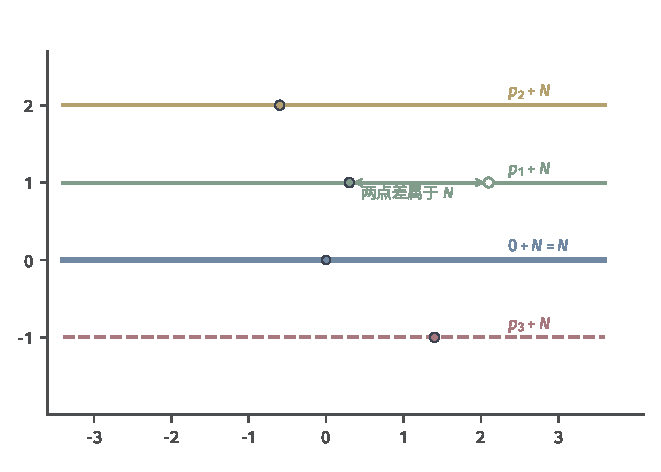
\includegraphics[width=112mm]{figures/00-shared/mathematical-preliminaries-upper/02-linear-spaces/matplotlib/ls-quotient-equivalence-classes/ls-quotient-equivalence-classes.pdf}
  \caption{商空间的等价类。$V=\mathbb R^2$，子空间$U$为$x$轴（蓝线$0+U$）；每条平行直线$p+U=\{(x,p_y)\}$是一个等价类，图中画出$y=1$（绿）、$y=2$（黄）、$y=-1$（红虚线）。绿线上实点$(0.3,1)$与空心点$(2.1,1)$之差$(1.8,0)\in U$，故属同一类；商空间$V/U$把每条平行线当成一个点。}
  \label{fig:ls-quotient-equivalence-classes}
\end{figure}

要让这些类像向量一样相加和缩放，自然的做法是对代表元作运算。
\begin{definition}[商空间]
\label{def:linear-algebra-quotient-space}
设$U$是线性空间$V$的子空间。全部等价类$\bm x+U$组成的集合记为$V/U$，规定
\[
 \begin{gathered}
(\bm x+U)+(\bm y+U)=(\bm x+\bm y)+U\\
a(\bm x+U)=a\bm x+U,
 \end{gathered}
\]
称$V/U$为$V$对$U$的\term{商空间}（quotient space）。
\end{definition}

借代表元定义运算，必须先检查结果与代表元的选取无关。把代表元换成$\bm x'=\bm x+\bm n_1$、$\bm y'=\bm y+\bm n_2$（$\bm n_1,\bm n_2\in U$）时，和与数乘的结果分别变成
\[
 \bm x'+\bm y'=(\bm x+\bm y)+(\bm n_1+\bm n_2),\qquad a\bm x'=a\bm x+a\bm n_1 ,
\]
只相差$\bm n_1+\bm n_2$与$a\bm n_1$。二者都属于$U$，所以得到的类不变。

零类是$U$本身，$\bm x+U$的相反类是$-\bm x+U$，其余规则由$V$的运算规则逐条继承，所以$V/U$是线性空间。在图~\ref{fig:ls-quotient-equivalence-classes}中，两条水平线相加就是高度相加：商空间只记录高度，忽略了沿$x$轴的位置。

商空间的元素是整条平行线，而不是从每条线上挑出的某个代表点。若在每条水平线上都取它与$y$轴的交点作代表，就等于另选了一个补空间（$y$轴）来记录各类；换成另一条过原点的非水平直线，代表点随之改变，类本身却不变。所以商空间描述的是“忽略$U$方向的差别以后剩下什么”，不依赖代表元或补空间的选择。

回到本节开头的截距问题，可以照此算出商空间的元素与运算。
\begin{example}[只保留截距的商空间]
\label{ex:ls-quotient-intercept}
取$V=P_1=\{a+bt:a,b\in\mathbb R\}$，要忽略的差别是斜率，所以取子空间$U=\{st:s\in\mathbb R\}$。

先看一个类里有哪些函数。$f_{a,b}=a+bt$所在的类是
\[
 f_{a,b}+U=\{a+(b+s)t:s\in\mathbb R\}=\{a+rt:r\in\mathbb R\},
\]
即截距为$a$、斜率任意的全部仿射函数，它只依赖$a$。

由此也可以判断两个类何时相同：$f_{a,b}+U=f_{a',b'}+U$当且仅当
\[
 f_{a,b}-f_{a',b'}=(a-a')+(b-b')t\in U,
\]
即$a=a'$。

再看运算。按商空间的定义，
\[
 \begin{gathered}
(f_{a,b}+U)+(f_{a',b'}+U)=f_{a+a',\,b+b'}+U\\
c(f_{a,b}+U)=f_{ca,\,cb}+U,
 \end{gathered}
\]
结果中的截距是$a+a'$与$ca$，即截距分别相加、缩放。

于是规则$f_{a,b}+U\mapsto a$是从$P_1/U$到$\mathbb R$的双射，并且保持加法与数乘。商空间$P_1/U$恰好只记录截距，斜率的差别已被忽略。
\end{example}
商空间的维数在第~\ref{sec:ls-dimension}节计算；它与线性映射的联系见第~\ref{sec:ls-kernel-image}节。

% 第2章第2节：基、维数与坐标（线性无关与张成、基、维数、坐标与坐标变换）。

\section{基、维数与坐标}
\label{sec:ls-bases-dimension-coordinates}

上一节规定了线性组合在什么范围内进行。本节用有限个数记录空间中的对象：选定一组方向，把对象写成它们的线性组合，再用组合系数代替对象。为此，先用张成与线性无关判断系数是否存在、是否唯一；两者同时成立的方向组称为基，基所含的向量个数就是空间的维数。最后定义基下的坐标，并推导换基时坐标怎样换算。

\subsection{张成与线性无关}

\paragraph{张成}
\phantomsection
\label{sec:ls-span}
在平面上，两个不共线方向的加权组合能取到每一个点；只有一个方向时，无论怎样加权，结果都停在过原点的一条直线上。为了描述一组方向能到达的范围，给它们的全部线性组合命名：给定$\bm v_1,\ldots,\bm v_k\in V$，集合
\begin{equation}
 \operatorname{span}\{\bm v_1,\ldots,\bm v_k\}
 =\left\{\sum_{j=1}^k a_j\bm v_j:a_j\in\mathbb R\right\}
 \label{eq:ls-span}
\end{equation}
称为这组向量的\term{张成空间}（span）。

两个线性组合再作线性组合，仍是这组向量的线性组合，所以张成空间对线性组合封闭，是$V$的子空间。

任何包含$\bm v_1,\ldots,\bm v_k$的子空间都必须含有它们的全部线性组合，所以张成空间是包含这组向量的最小子空间。若$\operatorname{span}\{\bm v_1,\ldots,\bm v_k\}=V$，就说这组向量张成$V$，也称它们是$V$的一个生成组。

在$\mathbb R^m$中，把$\bm v_1,\ldots,\bm v_k$排成矩阵$\bm V$的各列。按列读法，$\sum_ja_j\bm v_j=\bm V\bm a$，所以张成空间就是输出集合$\{\bm V\bm a:\bm a\in\mathbb R^k\}$。图~\ref{fig:ls-linear-combination-span}对比了两种情形：两个不共线方向的组合取遍整个平面，单个方向的组合只是一条直线。
\begin{figure*}[htbp]
  \centering
  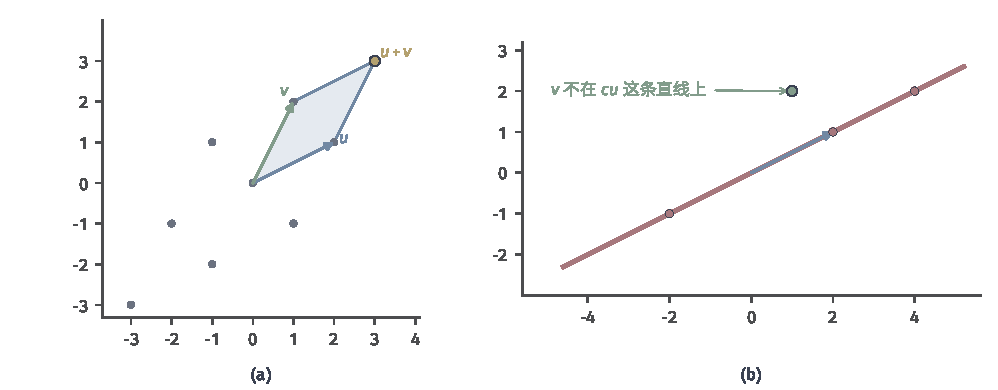
\includegraphics[width=169mm]{figures/00-shared/mathematical-preliminaries-upper/02-linear-spaces/matplotlib/ls-linear-combination-span/ls-linear-combination-span.pdf}
  \caption{两个方向与一个方向的张成范围。左：$\bm u=(2,1)$（蓝箭头）与$\bm v=(1,2)$（绿箭头）的全部加权组合取遍整个平面，浅蓝平行四边形标出$0,\bm u,\bm u+\bm v,\bm v$，灰点为整数系数格点，黄点为$\bm u+\bm v=(3,3)$。右：只有$\bm u$一个方向时，组合$\{c\bm u\}$只是过原点的一条直线（红线），$\bm v$不在其上。两图坐标等比例，为解析教学例。}
  \label{fig:ls-linear-combination-span}
\end{figure*}

\paragraph{线性无关}
\phantomsection
\label{sec:ls-linear-dependence}
张成回答“能表示哪些向量”，却不管“表示的方法有几种”。

先看一个平面上的例子。取
\[
 \bm u=(1,0)^\top,\qquad \bm v=(1,1)^\top,\qquad \bm w=(2,1)^\top .
\]
目标$(3,2)^\top$有两种写法：
\[
 (3,2)^\top=\bm u+2\bm v=\bm v+\bm w,
\]
两组系数$(1,2,0)$与$(0,1,1)$不同。原因是$\bm w=\bm u+\bm v$：$\bm w$能到达的地方，$\bm u$和$\bm v$合起来已经能到达，它没有带来新方向，只让系数多了一种选法。

把两种写法相减，得到
\[
 \bm u+\bm v-\bm w=\bm0 .
\]
这说明了一般规律：同一个向量若有两种不同的表示，相减就得到零向量的一个系数不全为零的表示；反过来，若零向量有这样的表示，把它加到任何一个表示上，就得到另一种表示。所以，要判断一组向量有没有多余的方向，只需看能否用不全为零的系数把它们组合成零向量。

据此给出定义。若
\begin{equation}
 a_1\bm v_1+\cdots+a_k\bm v_k=\bm0
 \label{eq:linear-algebra-independence-relation}
\end{equation}
只在$a_1=\cdots=a_k=0$时成立，就称$\bm v_1,\ldots,\bm v_k$\term{线性无关}（linearly independent）；否则称为\term{线性相关}（linearly dependent），即存在不全为零的系数使式~\eqref{eq:linear-algebra-independence-relation}成立。直观地说，线性无关就是“谁也不能被其余的向量凑出来”。

线性相关时，取一个非零系数$a_j$移项，就把$\bm v_j$写成其余向量的组合，如上例的$\bm w=\bm u+\bm v$；反之亦然。所以线性相关就是有某个向量多余，删去它不改变张成空间。

特别地，含零向量的组总是线性相关，两个向量线性相关当且仅当共线。在$\mathbb R^m$中，把向量排成矩阵$\bm V$的各列，线性无关就是$\bm V\bm a=\bm0$只有零解。上例的
\[
 \bm V=\begin{bmatrix}1&1&2\\0&1&1\end{bmatrix}
\]
有非零解$(1,1,-1)^\top$。

贯穿例中设计矩阵的两列几乎同向。它们是否线性无关，不能凭“看起来差不多”判断，要按定义检验。
\begin{example}[近共线的两列仍线性无关]
\label{ex:ls-nearly-collinear-independence}
式~\eqref{eq:linear-algebra-nearly-collinear-design}中的两列是$\bm c_1=(1,1,1)^\top$与$\bm c_2=\bm c_1+\varepsilon\bm q$，其中$\bm q=(0,1,-1)^\top$。$\bm c_2$由$\bm c_1$沿$\bm q$偏离一点得到，所以先确认$\bm c_1$与$\bm q$本身线性无关。二者的组合为
\[
 \alpha\bm c_1+\beta\bm q=(\alpha,\ \alpha+\beta,\ \alpha-\beta)^\top ,
\]
它为零时，第一坐标给出$\alpha=0$，第二坐标再给出$\beta=0$。

再把两列的组合改写到$\bm c_1,\bm q$上：
\[
 a_1\bm c_1+a_2\bm c_2=(a_1+a_2)\bm c_1+a_2\varepsilon\bm q .
\]
它为零时，由$\bm c_1,\bm q$线性无关，两个系数都须为零，即
\[
 a_1+a_2=0,\qquad a_2\varepsilon=0 .
\]
只要$\varepsilon\neq0$，第二式就迫使$a_2=0$，进而$a_1=0$，两列线性无关。只有$\varepsilon=0$时两列重合，$\bm c_1-\bm c_2=\bm0$，才线性相关。
\end{example}
因此，“几乎同向”与线性无关是两回事。线性无关只回答“是”或“否”：只要$\varepsilon\neq0$，答案就是“是”，不管$\varepsilon$多小。两列接近到什么程度，要用夹角等度量另行描述。

\paragraph{表示的存在与唯一}
张成管表示是否存在，线性无关管表示是否唯一，两者互不包含。下面的例子在平面上把它们分开。
\begin{example}[足够、不够与冗余的方向组]
\label{ex:ls-redundant-spanning-set}
在$\mathbb R^2$中取$\bm v_1=(1,0)^{\top}$、$\bm v_2=(0,1)^{\top}$与$\bm v_3=(1,1)^{\top}$，比较三种方向组。

用$\bm v_1,\bm v_2$两个方向时，$a_1\bm v_1+a_2\bm v_2=(a_1,a_2)^{\top}$，任一目标点$(x,y)^\top$都能取到，而且系数只能是$a_1=x$、$a_2=y$：方向既足够，又没有冗余。

只用$\bm v_1$时，组合$a_1\bm v_1=(a_1,0)^\top$停在横轴上，连$\bm v_2$都取不到：表示不一定存在。

三个方向一起用时，能到达的仍是整个平面，但$\bm v_3=\bm v_1+\bm v_2$，同一个目标有不同的系数，例如$(1,1)^\top$既是$\bm v_3$，又是$\bm v_1+\bm v_2$：表示存在，但不唯一。
\end{example}
图~\ref{fig:vol1-add-linear-redundant-directions}把第三种情形下的两种表示画在同一个平面上。
\begin{figure}[!htb]
  \centering
  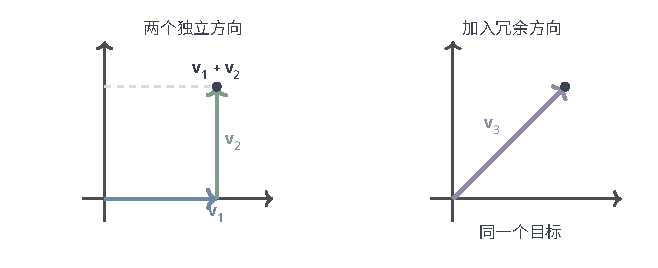
\includegraphics[width=112mm]{figures/00-shared/mathematical-preliminaries-upper/02-linear-spaces/tikz/comprehension-additions/linear-redundant-directions.pdf}
  \caption{冗余方向与重复表示。取$\bm v_1=(1,0)^{\top}$、$\bm v_2=(0,1)^{\top}$与$\bm v_3=(1,1)^{\top}$。左图沿$\bm v_1$再沿$\bm v_2$，右图直接沿$\bm v_3$，到达同一个目标；前两个向量已能表示平面中的每个向量，加入$\bm v_3$只使生成组冗余。两图坐标等比例。}
  \label{fig:vol1-add-linear-redundant-directions}
\end{figure}

一般地，张成保证每个向量都有表示；线性无关保证表示唯一，并且由上一段，表示唯一也反过来推出线性无关。后面定义坐标正以此为依据。

\subsection{基与维数}
\label{sec:ls-basis-dimension}

张成保证表示存在，线性无关保证表示唯一。同时满足这两个条件的一组向量称为\term{基}（basis）：它能到达整个空间，又没有多余的方向，可以充当整个空间的一把“尺子”。

$\mathbb R^d$的标准坐标向量$\bm e_1,\ldots,\bm e_d$是一组基，称为标准基：$\bm x=\sum_jx_j\bm e_j$说明它们张成$\mathbb R^d$，而$\sum_ja_j\bm e_j=(a_1,\ldots,a_d)^\top=\bm0$迫使全部$a_j=0$。

$P_k$中的$1,t,\ldots,t^k$也是一组基：每个多项式都是它们的组合，组合为零多项式时各项系数都为零。

子空间也有基。下面为一个齐次方程的解集合求出一组基。
\begin{example}[齐次方程解平面的一组基]
\label{ex:ls-solution-plane-basis}
设$N$是$\mathbb R^3$中齐次方程$x_1+2x_2+3x_3=0$的解集合；由示例~\ref{ex:ls-subspace-checks}，$N$是子空间。方程只约束了$x_1$：解满足
\[
 x_1=-2x_2-3x_3,
\]
而$x_2,x_3$可以任取。把每个解按这两个自由坐标拆开，
\[
 \bm x=x_2(-2,1,0)^\top+x_3(-3,0,1)^\top ,
\]
可见$\bm n_1=(-2,1,0)^\top$与$\bm n_2=(-3,0,1)^\top$张成$N$。

还要检查这两个方向没有冗余。若
\[
 a\bm n_1+b\bm n_2=(-2a-3b,\ a,\ b)^\top=\bm0,
\]
第二、三个坐标直接给出$a=b=0$，所以二者线性无关。于是$\bm n_1,\bm n_2$是$N$的一组基：两个自由坐标各对应一个基向量。
\end{example}

\paragraph{基的抽取与扩充}
若$V$有一个有限的生成组，就称$V$是有限维的；本章只讨论有限维空间。有限维空间总有基，可以从两个方向得到。

第一种做法是抽取。从任一有限生成组出发，若某个成员能写成其余向量的线性组合，删去它不会缩小张成范围。反复删除，直到剩下的向量中没有一个能由其余向量表示。这时剩下的向量线性无关，又仍张成$V$，构成一组基。

第二种做法是扩充。从任一线性无关组出发，逐次加入不在其张成空间中的向量。每加入一个新向量，张成范围严格扩大，新组仍线性无关。理由如下：若新组的某个组合为零，新向量的系数必为零，否则新向量能由原组表示，落在原张成空间中；新向量的系数为零以后，原组的线性无关性又使其余系数为零。

扩充不会无限进行下去。下文的交换引理（定理~\ref{thm:ls-exchange-lemma}）说明，有限维空间中线性无关组的长度不超过任一生成组的长度，所以扩充必在有限步内停止。停止时张成空间之外再没有向量，所得的组就是基。

抽取把冗余的生成组压缩成基，扩充把线性无关组补足成基。后面的许多证明都会用到扩充。

\paragraph{维数}
\label{sec:ls-dimension}

基的向量个数可以度量空间的大小，前提是换一组基时个数不变。这由交换引理保证。
\begin{theorem}[交换引理]
\label{thm:ls-exchange-lemma}
若$\bm u_1,\ldots,\bm u_r$线性无关，且每个$\bm u_i$都属于$\operatorname{span}\{\bm v_1,\ldots,\bm v_s\}$，则$r\leq s$；并且这$r$个$\bm u_i$可以逐个换入原生成组、换出同样多个$\bm v_j$，每次换完新组仍张成原来的空间。
\end{theorem}
\begin{proof}
从生成组$G_0=\{\bm v_1,\ldots,\bm v_s\}$开始。

因为$\bm u_1\in\operatorname{span}G_0$，它可写成若干$\bm v_j$的组合。这些系数不全为零，否则$\bm u_1=\bm0$，与$\bm u_1,\ldots,\bm u_r$线性无关矛盾。

取某个系数非零的$\bm v_j$，从这个表达式中把它解出，$\bm v_j$就能由$\bm u_1$与其余的$\bm v$表示。于是用$\bm u_1$换出$\bm v_j$，新组$G_1$与$G_0$张成同一个空间。

一般地，设第$i-1$步后的组$G_{i-1}$由$\bm u_1,\ldots,\bm u_{i-1}$和$s-(i-1)$个留下的$\bm v$组成，且与$G_0$张成同一空间。于是$\bm u_i\in\operatorname{span}G_{i-1}$。若$\bm u_i$只用$\bm u_1,\ldots,\bm u_{i-1}$就能表示，就违反线性无关；所以表达式中至少有一个留下的$\bm v$系数非零。把它解出并换入$\bm u_i$，张成范围不变。只要还有留下的$\bm v$，这一步就能继续。

若$r>s$，换满$s$次以后组内只剩$\bm u_1,\ldots,\bm u_s$，而$\bm u_{s+1}$属于$\operatorname{span}G_s=\operatorname{span}\{\bm u_1,\ldots,\bm u_s\}$，与$r$个$\bm u$线性无关矛盾。

故$r\leq s$，上面的逐次交换就是定理所说的换入换出过程。
\end{proof}

由交换引理，基的向量个数与基的选取无关。任取两组基，设个数分别为$r$与$s$。把第一组看成线性无关组、第二组看成生成组，得$r\leq s$；互换两组的角色，又得$s\leq r$，所以$r=s$。

这个共同的个数称为空间的\term{维数}（dimension），记为$\dim V$。只含零向量的空间以空集为基，维数为$0$。

交换引理的论证依赖有限的生成组，所以后面的基扩充与维数计算都限于有限维空间，不能直接用于无限维的函数展开。

\subsection{子空间的维数与分解}
有了维数，就能比较子空间的大小。若$U\subseteq W$，取$U$的一组基，它在$W$中仍线性无关，可以按上一小节的方法扩充成$W$的基。扩充只增加向量，所以$\dim U\leq\dim W$；新增向量的个数恰为$\dim W-\dim U$，它表示$U$之外还有多少个独立方向。

若同时有$\dim U=\dim W$，把$U$的基扩充成$W$的基不需要新增向量，即$U$的基已经张成$W$，所以$U=W$。这里的包含条件不能省略，仅凭维数相同推不出包含。
\begin{example}[反例：同维而互不包含的两条直线]
\label{ex:ls-equal-dimension-not-nested}
在$\mathbb R^2$中取横轴$U=\{(s,0)^\top:s\in\mathbb R\}$与对角线$W=\{(s,s)^\top:s\in\mathbb R\}$。二者分别以$\bm e_1$与$(1,1)^\top$为基，所以$\dim U=\dim W=1$。

然而$\bm e_1$的两个坐标不相等，不在$W$中；$(1,1)^\top$的第二坐标不为零，也不在$U$中。

两条直线维数相同，却互不包含。维数只数方向的个数，不记录这些方向指向哪里，所以上面的结论必须以$U\subseteq W$为前提。
\end{example}
“先取已有的基，再补新方向”这一做法，下面计算和空间、补空间与商空间时都会用到，后面的秩零度定理也以它为证明思路。

\paragraph{和空间}
两个子空间的公共方向在两边各计一次，所以和空间的维数一般小于两边维数之和。下面从交的一组基出发，算出准确的公式。

设$\bm z_1,\ldots,\bm z_k$是$U\cap W$的一组基，把它扩充为$U$的基$\bm z_1,\ldots,\bm z_k,\bm u_1,\ldots,\bm u_p$，再另行扩充为$W$的基$\bm z_1,\ldots,\bm z_k,\bm w_1,\ldots,\bm w_q$。我们说明这$k+p+q$个向量构成$U+W$的基。

每个$\bm u+\bm w$（$\bm u\in U$，$\bm w\in W$）都是这些向量的组合，所以它们张成$U+W$。为证线性无关，设
\[
 \sum_i\alpha_i\bm z_i+\sum_j\beta_j\bm u_j+\sum_l\gamma_l\bm w_l=\bm0 .
\]
移项得
\[
 \sum_l\gamma_l\bm w_l=-\sum_i\alpha_i\bm z_i-\sum_j\beta_j\bm u_j .
\]
左边属于$W$，右边属于$U$，所以这个向量属于$U\cap W$，可以写成$\sum_i\delta_i\bm z_i$。于是
\[
 \sum_l\gamma_l\bm w_l-\sum_i\delta_i\bm z_i=\bm0,
\]
由$W$的基线性无关，全部$\gamma_l=0$。代回原式，再由$U$的基线性无关，全部$\alpha_i$与$\beta_j$也为零。

因此
\[
 \dim(U+W)=k+p+q=(k+p)+(k+q)-k,
\]
即
\begin{equation}
 \dim(U+W)=\dim U+\dim W-\dim(U\cap W).
 \label{eq:ls-dimension-formula}
\end{equation}
减去的是两边重复计入的公共方向的个数，不是两个集合元素个数之差。下面在$\mathbb R^3$中核对这一公式。
\begin{example}[两个坐标平面的和]
\label{ex:ls-dimension-formula-planes}
在$\mathbb R^3$中取两个坐标平面$U=\operatorname{span}\{\bm e_1,\bm e_2\}$与$W=\operatorname{span}\{\bm e_2,\bm e_3\}$，维数都是$2$。

先求交：$U$由第三坐标为零的向量组成，$W$由第一坐标为零的向量组成，同时满足两条的向量只剩第二坐标，所以$U\cap W=\operatorname{span}\{\bm e_2\}$，维数为$1$。

再看和：$U+W$含有$\bm e_1,\bm e_2,\bm e_3$，所以就是$\mathbb R^3$。两边与公式相符：
\[
 \dim(U+W)=3=2+2-1 .
\]
减去的$1$正是两个平面共有的$\bm e_2$方向，它在$\dim U$与$\dim W$中各计了一次。

作为对照，改取两条坐标轴$U'=\operatorname{span}\{\bm e_1\}$、$W'=\operatorname{span}\{\bm e_2\}$。它们没有公共的非零向量，交为零，于是
\[
 \dim(U'+W')=1+1-0=2 .
\]
交为零时，和的维数等于两边维数之和。
\end{example}

\paragraph{补空间}
第~\ref{sec:ls-direct-sum}节定义了补空间，现在用基扩充证明它总存在。把$U$的基扩充为$V$的基，新增向量张成的子空间记为$W$。整组基张成$V$，所以$U+W=V$。

若某个向量同属$U$与$W$，它既是$U$的基向量的组合，又是新增向量的组合；两种写法相减，得到整组基的一个组合为零，所以系数全为零，该向量为零。于是$U\cap W=\{\bm0\}$，$V=U\oplus W$。

由维数公式，直和时交的维数为零，所以$\dim V=\dim U+\dim W$。扩充的方式不唯一，补空间也就不唯一，这与平面中直线的例子一致。

\paragraph{商空间}
同样的扩充也给出第~\ref{sec:ls-quotient-spaces}节商空间的维数。取$U$的一组基$\bm u_1,\ldots,\bm u_s$，扩充为$V$的基$\bm u_1,\ldots,\bm u_s,\bm w_1,\ldots,\bm w_t$。新增向量的类$\bm w_1+U,\ldots,\bm w_t+U$张成$V/U$：任一$\bm x$写成整组基的组合，其中属于$U$的部分落进零类而消去。

这些类也线性无关。若$\sum_ja_j(\bm w_j+U)=U$，则$\sum_ja_j\bm w_j\in U$，它能由$\bm u_i$表示，整组基的线性无关性迫使全部$a_j=0$。因此
\begin{equation}
 \dim(V/U)=\dim V-\dim U.
 \label{eq:ls-quotient-dimension}
\end{equation}

商空间的维数等于补空间的维数，二者的关系还可以说得更具体。新增向量$\bm w_j$张成$U$的一个补空间$W$，每个$\bm x$唯一分解为
\[
 \bm x=\bm u+\bm w,\qquad \bm u\in U,\ \bm w\in W,
\]
于是类$\bm x+U=\bm w+U$中的点都形如$\bm w+\bm u'$（$\bm u'\in U$）。这样的点落在$W$中，当且仅当$\bm u'\in U\cap W=\{\bm0\}$，所以每个类与$W$恰交于一点$\bm w$。

选定一个补空间，就是为每个类选定一个代表元。补空间需要选择，商空间不依赖任何选择，这是二者的区别。

在示例~\ref{ex:ls-quotient-intercept}中，$\dim(P_1/U)=2-1=1$，商空间只剩截距这一个方向；在图~\ref{fig:ls-quotient-equivalence-classes}中，$\dim(\mathbb R^2/U)=1$，只剩高度。

\subsection{坐标与坐标变换}
\label{sec:ls-coordinates}
\label{sec:linear-algebra-coordinates}

有了基，每个对象都有唯一的一组系数。本小节先把这组系数定义为坐标，说明它怎样代替对象参与计算；再看坐标的大小为什么不能直接反映对象的大小；最后推导换基时坐标的换算规则。

\paragraph{有序基下的坐标}
固定有序基$\mathcal B=(\bm b_1,\ldots,\bm b_d)$后，对象$\bm v$唯一写成$\sum_{j=1}^d x_j\bm b_j$。系数列$[\bm v]_{\mathcal B}=(x_1,\ldots,x_d)^{\top}$称为$\bm v$在基$\mathcal B$下的\term{坐标}（coordinates）。

由于存在性来自张成、唯一性来自线性无关，坐标映射$\bm v\mapsto[\bm v]_{\mathcal B}$是从$V$到$\mathbb R^d$的双射：每个对象恰有一列坐标，每列实数$(x_1,\ldots,x_d)^{\top}$也恰好记录对象$\sum_jx_j\bm b_j$。

坐标映射还保持线性组合。若$[\bm v]_{\mathcal B}=\bm x$、$[\bm w]_{\mathcal B}=\bm y$，则$a\bm v+b\bm w=\sum_j(ax_j+by_j)\bm b_j$，由唯一性得
\[
 [a\bm v+b\bm w]_{\mathcal B}=a\bm x+b\bm y.
\]
因此，对象上的线性运算可以完全在坐标上进行，算完再按基还原。

在$\mathbb R^d$中，把基向量排成矩阵$\bm B=[\bm b_1\ \cdots\ \bm b_d]$。按列读法，$\bm v=\bm B[\bm v]_{\mathcal B}$，所以坐标就是方程$\bm B\bm x=\bm v$的唯一解。下面用这个方程求一个斜基下的坐标。
\begin{example}[同一向量在两组基下的坐标]
\label{ex:ls-coordinates-two-bases}
取$\mathbb R^2$中的向量$\bm x=(1,2)^\top$。在标准基$(\bm e_1,\bm e_2)$下，$\bm x=1\cdot\bm e_1+2\cdot\bm e_2$，坐标就是$(1,2)^\top$。改用斜基$\mathcal B=(\bm b_1,\bm b_2)$，其中$\bm b_1=(2,1)^\top$、$\bm b_2=(-1,1)^\top$，坐标$(c_1,c_2)^\top$要由$c_1\bm b_1+c_2\bm b_2=\bm x$解出，逐坐标写开就是
\[
 \begin{gathered}
2c_1-c_2=1\\
c_1+c_2=2 .
 \end{gathered}
\]
两式相加消去$c_2$，得$3c_1=3$，所以$c_1=1$，再代入第二式得$c_2=1$。代回检验，
\[
 \bm b_1+\bm b_2=(1,2)^\top
\]
正是$\bm x$。

所以$[\bm x]_{\mathcal B}=(1,1)^\top$。向量本身没有移动，只是换了一组基来度量，读数随之改变。
\end{example}
图~\ref{fig:ls-basis-coordinates}画出这两种读法。
\begin{figure*}[htbp]
  \centering
  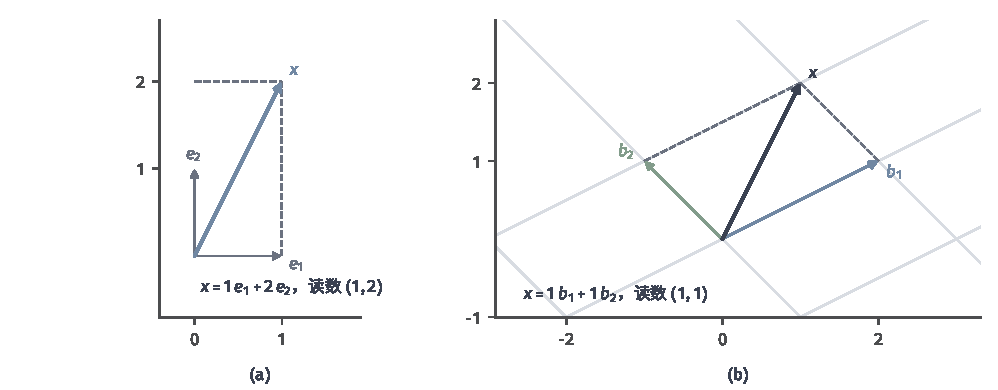
\includegraphics[width=169mm]{figures/00-shared/mathematical-preliminaries-upper/02-linear-spaces/matplotlib/ls-basis-coordinates/ls-basis-coordinates.pdf}
  \caption{同一向量在两组基下的坐标。左：标准基$\bm e_1,\bm e_2$（灰箭头）下，向量$\bm x=(1,2)$（蓝箭头）的坐标为$(1,2)$，虚线为向坐标轴的垂线。右：斜基$\bm b_1=(2,1)$（蓝）、$\bm b_2=(-1,1)$（绿）下，同一个$\bm x$满足$\bm x=\bm b_1+\bm b_2$，坐标为$(1,1)$，浅色斜线为斜基网格，虚线为平行四边形读法。两图坐标系相同。}
  \label{fig:ls-basis-coordinates}
\end{figure*}

\paragraph{坐标与对象}
坐标要与它记录的对象区分开。几何位移、有限信号、多项式都可以相加和缩放，它们是\emph{对象}；一列实数只是选定基以后记录对象的\emph{坐标}。基的顺序也要固定：交换$\bm b_1,\bm b_2$，对象不变，坐标列的前两个数随之交换。

在$\mathbb R^d$中直接写一列数，通常默认使用标准基$\bm e_1,\ldots,\bm e_d$，这时对象与坐标恰好是同一列数。第~\ref{chap:linear-operations}章就是在这种默认下工作的。

对函数的基展开，二者必须分开：函数是对象，展开系数是坐标。
\begin{example}[仿射函数在两组基下的坐标]
\label{ex:ls-affine-function-coordinates}
在$P_1$中用两组基记录同一个仿射函数$f_{a,b}=a+bt$。在$\mathcal B_1=(1,t)$下，$f_{a,b}=a\cdot1+b\cdot t$，坐标就是截距与斜率$(a,b)^\top$。

换成$\mathcal B_2=(1,1+t)$，设
\[
 f_{a,b}=c_1\cdot1+c_2(1+t)=(c_1+c_2)+c_2t ;
\]
比较$t$的系数得$c_2=b$，再比较常数项得$c_1=a-b$，即
\[
 f_{a,b}=(a-b)\cdot1+b\cdot(1+t).
\]
同一个函数在$\mathcal B_1$与$\mathcal B_2$下的坐标分别是$(a,b)^\top$与$(a-b,b)^\top$。坐标改变了，函数本身没有改变；“截距是第一个坐标”只在$\mathcal B_1$下成立。
\end{example}
坐标的个数总等于维数。若用冗余的生成组记录对象，记录的长度可以超过维数，所以不能由这种记录的长度推断空间的维数。

\paragraph{坐标对基的敏感性}
对象不变时，不同基下的坐标仍可能相差很大。贯穿例给出一个极端的情形。
\begin{example}[近共线基下的大坐标]
\label{ex:ls-coordinate-instability}
沿用示例~\ref{ex:ls-nearly-collinear-independence}中的$\bm c_1,\bm q$与$\bm c_2=\bm c_1+\varepsilon\bm q$（$\varepsilon\neq0$），并取$\delta=0.1$与目标向量
\begin{equation}
 \bm y=\bm c_1+\delta\bm q=\begin{bmatrix}1\\1.1\\0.9\end{bmatrix}.
 \label{eq:linear-algebra-nearly-collinear-target}
\end{equation}
由该示例，$\mathcal B_0=(\bm c_1,\bm q)$与$\mathcal B_\varepsilon=(\bm c_1,\bm c_2)$都是平面$\operatorname{span}\{\bm c_1,\bm q\}$的基，$\bm y$也在这个平面中，所以可以比较它在两组基下的坐标。

在$\mathcal B_0$下，$\bm y$的坐标直接读出为$(1,\delta)^{\top}$。要换到$\mathcal B_\varepsilon$，先由$\bm c_2=\bm c_1+\varepsilon\bm q$解出$\bm q=(\bm c_2-\bm c_1)/\varepsilon$，再代入$\bm y=\bm c_1+\delta\bm q$，得
\begin{equation}
 \bm y=\left(1-\frac{\delta}{\varepsilon}\right)\bm c_1
       +\frac{\delta}{\varepsilon}\bm c_2.
 \label{eq:linear-algebra-coordinate-instability}
\end{equation}
两个系数都含因子$\delta/\varepsilon$，$\varepsilon$越小，坐标越大。取$\varepsilon=0.01$，则$\delta/\varepsilon=10$，坐标成为$(-9,10)^{\top}$。

于是同一个$\bm y$在两组基下的坐标为
\[
 [\bm y]_{\mathcal B_0}=(1,0.1)^\top,\qquad [\bm y]_{\mathcal B_{0.01}}=(-9,10)^\top,
\]
第二个分量从$0.1$变成了$10$。
\end{example}
两个很大的系数作用在几乎同向的两个基向量上，大部分相互抵消，所以不能据此判断$\bm y$很大。坐标对接近退化的基的这种敏感性，第~\ref{chap:condition-and-spectral-perturbation}章将用条件数定量讨论。要系统地比较新旧坐标，先要建立换基的一般公式。

\paragraph{换基矩阵}
\phantomsection
\label{sec:ls-change-basis}
\label{sec:linear-algebra-coordinate-conversions}
设$\mathcal B=(\bm b_1,\ldots,\bm b_d)$与$\mathcal C$是$V$的两组有序基，已知$\bm v$在$\mathcal B$下的坐标$[\bm v]_{\mathcal B}=(x_1,\ldots,x_d)^{\top}$，要求它在$\mathcal C$下的坐标。由$\bm v=\sum_jx_j\bm b_j$，并且坐标映射保持线性组合，
\[
 [\bm v]_{\mathcal C}=\sum_{j=1}^d x_j[\bm b_j]_{\mathcal C}.
\]
右边是各列$[\bm b_j]_{\mathcal C}$以$x_j$为权重的线性组合。把这些列排成矩阵，称为从$\mathcal B$到$\mathcal C$的换基矩阵$\bm S_{\mathcal C\leftarrow\mathcal B}$。按矩阵与向量乘积的列读法，
\begin{equation}
 [\bm v]_{\mathcal C}
 =\bm S_{\mathcal C\leftarrow\mathcal B}[\bm v]_{\mathcal B}.
 \label{eq:linear-algebra-coordinate-change}
\end{equation}
换基矩阵的第$j$列是旧基向量$\bm b_j$的新坐标。下标$\mathcal C\leftarrow\mathcal B$从右向左读，表示把$\mathcal B$坐标换算成$\mathcal C$坐标。下面在平面上算一个具体的换基矩阵。
\begin{example}[平面上的换基矩阵]
\label{ex:ls-change-of-basis-plane}
设$\mathbb R^2$中的向量$\bm v$在基$\mathcal U=(\bm u_1,\bm u_2)$下的坐标为$(1,1)^\top$，其中$\bm u_1=(1,0)^{\top}$、$\bm u_2=(1,1)^{\top}$，要求它在标准基$\mathcal E$下的坐标。这里$\mathcal U$是旧基，$\mathcal E$是新基；$\bm u_1,\bm u_2$的标准坐标就是它们自己，按“第$j$列是旧基向量的新坐标”排成
\[
 \bm S_{\mathcal E\leftarrow\mathcal U}=\begin{bmatrix}1&1\\0&1\end{bmatrix}.
\]
由式~\eqref{eq:linear-algebra-coordinate-change}，
\[
 [\bm v]_{\mathcal E}=\bm S_{\mathcal E\leftarrow\mathcal U}(1,1)^{\top}=(2,1)^{\top}.
\]
不用换基矩阵也能得到同样结果：
\[
 \bm v=\bm u_1+\bm u_2=(2,1)^\top .
\]
所以$\mathcal U$坐标$(1,1)^\top$与标准坐标$(2,1)^\top$记录的是同一个向量。
\end{example}
图~\ref{fig:vol1-add-linear-change-basis}画出这一点：目标位置没有移动，改变的只是沿哪两个基方向累加，以及每个方向取多少份。
\begin{figure}[!htb]
  \centering
  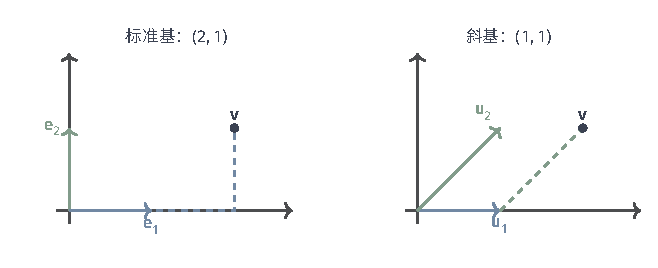
\includegraphics[width=112mm]{figures/00-shared/mathematical-preliminaries-upper/02-linear-spaces/tikz/comprehension-additions/linear-change-basis.pdf}
  \caption{同一向量的两套坐标。左图使用标准基，$\bm v=(2,1)^{\top}$的坐标为$(2,1)^{\top}$；右图使用$\bm u_1=(1,0)^{\top}$、$\bm u_2=(1,1)^{\top}$，同一$\bm v$的坐标为$(1,1)^{\top}$。虚线表示相应的向量相加，两图的环境坐标比例相同。}
  \label{fig:vol1-add-linear-change-basis}
\end{figure}

\paragraph{连续换基与反向换基}
连续换两次基，结果应与直接换基相同。设还有第三组基$\mathcal D$。对每个$\bm v$，连用两次式~\eqref{eq:linear-algebra-coordinate-change}，
\[
 \begin{aligned}
 [\bm v]_{\mathcal D}&=\bm S_{\mathcal D\leftarrow\mathcal C}[\bm v]_{\mathcal C}\\
 &=\bm S_{\mathcal D\leftarrow\mathcal C}\bm S_{\mathcal C\leftarrow\mathcal B}[\bm v]_{\mathcal B}.
 \end{aligned}
\]
取$\bm v=\bm b_j$，它的$\mathcal B$坐标是$\bm e_j$，两边读出的分别是$\bm S_{\mathcal D\leftarrow\mathcal B}$与乘积的第$j$列，所以
\[
 \bm S_{\mathcal D\leftarrow\mathcal B}
 =\bm S_{\mathcal D\leftarrow\mathcal C}\bm S_{\mathcal C\leftarrow\mathcal B}.
\]

特别取$\mathcal D=\mathcal B$。每个$\bm b_j$在$\mathcal B$下的坐标是$\bm e_j$，所以$\bm S_{\mathcal B\leftarrow\mathcal B}=\bm I_d$，即
\[
 \bm S_{\mathcal B\leftarrow\mathcal C}\bm S_{\mathcal C\leftarrow\mathcal B}=\bm I_d ;
\]
交换两组基的角色，同理得
\[
 \bm S_{\mathcal C\leftarrow\mathcal B}\bm S_{\mathcal B\leftarrow\mathcal C}=\bm I_d .
\]
所以换基矩阵总可逆，反向换基矩阵就是它的逆：
\[
 \bm S_{\mathcal B\leftarrow\mathcal C}=\bm S_{\mathcal C\leftarrow\mathcal B}^{-1}.
\]
在示例~\ref{ex:ls-change-of-basis-plane}中，
\[
 \bm S_{\mathcal U\leftarrow\mathcal E}=\bm S_{\mathcal E\leftarrow\mathcal U}^{-1}=\begin{bmatrix}1&-1\\0&1\end{bmatrix},
\]
它把$(2,1)^{\top}$送回$(1,1)^{\top}$。

反过来，任一$d$阶可逆矩阵$\bm P$都是某次换基的矩阵。以$\bm P$的第$j$列为$\mathcal B$坐标，取向量$\bm b'_j=\sum_i\bm P_{i,j}\bm b_i$。$\bm P$的列线性无关，而坐标映射是保持线性组合的双射，所以$\bm b'_1,\ldots,\bm b'_d$也线性无关。

个数等于维数的线性无关组必是基：否则它还能扩充，得到多于$\dim V$个线性无关的向量，与交换引理矛盾。于是$\bm b'_1,\ldots,\bm b'_d$构成一组基$\mathcal B'$。按定义，$\bm S_{\mathcal B\leftarrow\mathcal B'}$的第$j$列是$\bm b'_j$的$\mathcal B$坐标，即$\bm P$的第$j$列，所以$\bm S_{\mathcal B\leftarrow\mathcal B'}=\bm P$。

换基矩阵接近不可逆时，反向换基会放大坐标。贯穿例清楚地显示了这一点。
\begin{example}[近共线基之间的换基]
\label{ex:ls-nearly-collinear-change-of-basis}
回到示例~\ref{ex:ls-coordinate-instability}中的两组基$\mathcal B_0=(\bm c_1,\bm q)$与$\mathcal B_\varepsilon=(\bm c_1,\bm c_2)$，$\varepsilon\neq0$，用换基矩阵重做那里的坐标换算。由
\[
 \bm c_1=1\cdot\bm c_1+0\cdot\bm q,\qquad \bm c_2=1\cdot\bm c_1+\varepsilon\bm q,
\]
$\mathcal B_\varepsilon$的两个向量在$\mathcal B_0$下的坐标分别是$(1,0)^{\top}$与$(1,\varepsilon)^{\top}$。以它们为列得到$\bm S_{\mathcal B_0\leftarrow\mathcal B_\varepsilon}$，求逆得到反方向的换基矩阵：
\[
\begin{gathered}
\bm S_{\mathcal B_0\leftarrow\mathcal B_\varepsilon}
 =\begin{bmatrix}1&1\\0&\varepsilon\end{bmatrix}\\
\bm S_{\mathcal B_\varepsilon\leftarrow\mathcal B_0}
 =\bm S_{\mathcal B_0\leftarrow\mathcal B_\varepsilon}^{-1}
 =\begin{bmatrix}1&-1/\varepsilon\\0&1/\varepsilon\end{bmatrix},
\end{gathered}
\]
逆矩阵可由两者相乘得单位矩阵验证。把$\bm y$在$\mathcal B_0$下的坐标$(1,\delta)^{\top}$代入后者，得
\[
 \bm S_{\mathcal B_\varepsilon\leftarrow\mathcal B_0}\begin{bmatrix}1\\\delta\end{bmatrix}
 =\begin{bmatrix}1-\delta/\varepsilon\\\delta/\varepsilon\end{bmatrix},
\]
与式~\eqref{eq:linear-algebra-coordinate-instability}一致。

放大的来源在矩阵上看得很清楚。$\bm S_{\mathcal B_0\leftarrow\mathcal B_\varepsilon}$的行列式为$\varepsilon$，接近零，矩阵接近不可逆；它的逆因而含有因子$1/\varepsilon$，两组基之间的微小差异由此被放大成大系数。
\end{example}

\paragraph{被动换基与主动作用}
换基公式与矩阵作用都写成矩阵乘以坐标列，但含义不同，必须分开。换基是被动的：对象不动，记录改变，式\eqref{eq:linear-algebra-coordinate-change}两侧是同一个$\bm v$的两套坐标。矩阵作用是主动的：坐标系不动，对象被送到另一个对象，例如第~\ref{chap:linear-operations}章的$\bm x\mapsto\bm A\bm x$把向量旋转或切变；下一节把这种作用推广为线性映射。下面的例子从同一个初始向量出发比较两种情形。
\begin{example}[被动换基与主动切变]
\label{ex:ls-passive-vs-active}
取$\mathbb R^2$中的向量$\bm x=(3,3)^\top$，分别对它作被动换基与主动切变。换基用斜基$\mathcal B'=(\bm b_1,\bm b_2)$，$\bm b_1=(2,1)^\top$、$\bm b_2=(-1,1)^\top$；切变用矩阵
\[
 \bm A=\begin{bmatrix}1&1\\0&1\end{bmatrix}.
\]

被动换基要求$\bm x$在$\mathcal B'$下的坐标$(c_1,c_2)^\top$。逐坐标写开得
\[
 \begin{gathered}
 2c_1-c_2=3\\
 c_1+c_2=3,
 \end{gathered}
\]
解得$c_1=2$、$c_2=1$，即$\bm x=2\bm b_1+\bm b_2$。这时向量仍是$(3,3)^\top$，只是读数从$(3,3)$变成$(2,1)$。

主动作用则在标准坐标下计算
\[
 \bm A\bm x=(3+3,\ 3)^\top=(6,3)^\top .
\]
这时坐标系不动，向量本身被搬到了另一个位置。
\end{example}
图~\ref{fig:ls-passive-change-vs-active-map}把两种情形并排画出。可见，并非所有乘矩阵的运算都是换基。
\begin{figure*}[htbp]
  \centering
  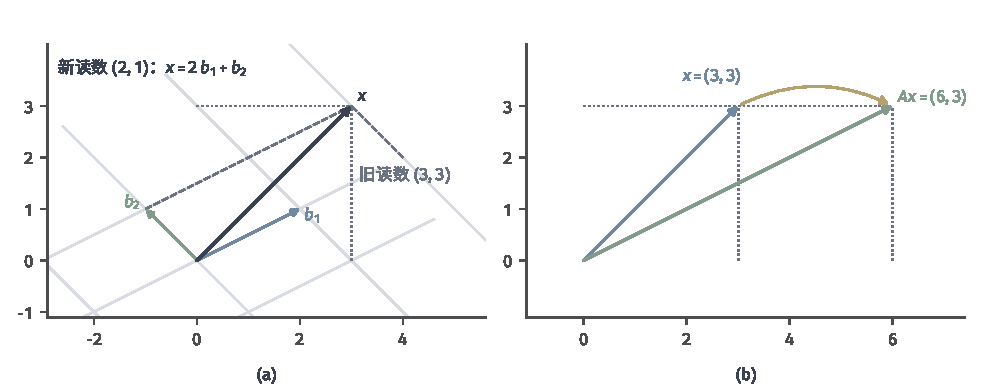
\includegraphics[width=169mm]{figures/00-shared/mathematical-preliminaries-upper/02-linear-spaces/matplotlib/ls-passive-change-vs-active-map/ls-passive-change-vs-active-map.pdf}
  \caption{被动换基与主动变换的对照，两图使用同一个初始向量$\bm x=(3,3)$。左（被动换基）：箭头位置不动（深色），旧标准读数用点线投影读出$(3,3)$；新斜基$\bm b_1=(2,1)$（蓝）、$\bm b_2=(-1,1)$（绿）与浅色斜网格下，$\bm x=2\bm b_1+\bm b_2$，新读数为$(2,1)$。右（主动变换）：标准坐标系不动，$\bm x$（蓝）被切变映到$\bm A\bm x=(6,3)$（绿），黄色弧线表示搬动过程。}
  \label{fig:ls-passive-change-vs-active-map}
\end{figure*}

% 第2章第3节：线性映射（定义；表示：矩阵表示、基于矩阵的映射运算、矩阵基本子空间；核与像、秩零度、商空间、行空间与列空间、可逆性；换基：相抵与相似；多线性映射）。

\section{线性与多线性映射}
\label{sec:ls-linear-maps}
\label{sec:linear-algebra-matrices-linear-maps}

前两节讨论单个空间中的对象怎样记录。本节转向对象之间保持线性组合的作用，即线性映射。选定两端的基，线性映射记成矩阵，映射的叠加、复合与求逆对应矩阵的加法、乘法与求逆。核与像分别描述映射消去的输入和能到达的输出，秩零度定理联系二者的维数，并由此给出可逆的判据。换基改变矩阵而不改变映射：两端各自换基得到相抵，算子两端同时换基得到相似。最后简述对每个输入分别线性的多线性映射。

\subsection{线性映射及其矩阵表示}
\label{sec:ls-linear-map-definition}
\label{sec:linear-algebra-maps}

设计矩阵把一组系数变成一列拟合值，求导把一个多项式变成另一个多项式，读取第一个坐标把向量变成一个数。这些作用有一个共同点：先把输入加权相加再作用，与先分别作用再作同样的加权相加，结果相同。有了这一性质，输入写成基向量的组合以后，作用的结果就是各基向量的像的同样组合，前两节的语言可以直接用于作用本身。保持线性组合的作用称为\term{线性映射}（linear map）$T:V\to W$：
\begin{equation}
T(a\bm x+b\bm y)=aT\bm x+bT\bm y,\qquad\bm x,\bm y\in V,\ a,b\in\mathbb R.
\label{eq:ls-linear-map-def}
\end{equation}
取$a=b=0$得$T\bm0=\bm0$，线性映射总把零向量送到零向量。由式~\eqref{eq:prelim-matrix-linearity}，任何矩阵$\bm A\in\mathbb R^{m\times d}$给出的$\bm x\mapsto\bm A\bm x$都是从$\mathbb R^d$到$\mathbb R^m$的线性映射。下面再检查几个作用是否线性。
\begin{example}[线性与非线性的作用]
\label{ex:ls-linear-map-checks}
考察下面三个作用：
\[
 \begin{aligned}
 &T:\mathbb R^2\to\mathbb R^2, &&T(x_1,x_2)=(2x_1+x_2,\ 3x_2);\\
 &D:P_k\to P_k, &&Dp=p';\\
 &\tau:\mathbb R\to\mathbb R, &&\tau(x)=x+1.
 \end{aligned}
\]
$T$的两个输出分量都是输入的加权和，写成矩阵就是
\[
 T\bm x=\begin{bmatrix}2&1\\0&3\end{bmatrix}\bm x,
\]
所以它是矩阵给出的映射，保持线性组合。求导满足$(ap+bq)'=ap'+bq'$，所以$D$也保持线性组合；又因为求导不升高次数，$D$确实把$P_k$送回$P_k$。

$\tau$看起来同样简单，却不是线性映射：$\tau(0)=1\neq0$，而线性映射必把$0$送到$0$。加上常数就把零点移走了，这与示例~\ref{ex:ls-subspace-checks}中平移后的直线不含零向量是同一类现象。
\end{example}

\phantomsection
\label{sec:ls-operator-powers}
输入与输出是同一个空间的线性映射$T:V\to V$称为\term{线性算子}（linear operator），也称线性变换。平面上的旋转、向一条直线的投影、$P_k$上的求导都是线性算子，示例~\ref{ex:ls-linear-map-checks}中的$T$也是。

输入与输出相同，使算子与一般映射有两点不同。第一，算子的输出仍在$V$中，可以再次作为输入，所以算子能与自身复合、反复作用。记$T^2=T\circ T$、$T^k=T\circ T^{k-1}$，并约定$T^0=\operatorname{id}_V$。一般映射$V\to W$在$V\neq W$时不能这样反复作用。后面将看到，在同一组基下，$T^k$的矩阵就是$T$的矩阵的$k$次幂。

第二，记录算子时，输入和输出可以用同一组基，这决定了算子换基时的特殊规律（第~\ref{sec:ls-similarity}节）。

\phantomsection
\label{sec:ls-map-representation}
线性映射的定义域通常有无穷多个元素，不可能逐个记录输出。选定基以后，有限个数就够了：在两端的固定基下，线性映射与矩阵一一对应，映射的叠加、复合与求逆分别对应矩阵的加法、乘法与求逆。第~\ref{chap:linear-operations}章的矩阵由此获得一般含义：矩阵是线性映射在坐标下的记录。下面先建立这一对应，再翻译映射的运算，最后定义矩阵的四个基本子空间，供下一小节使用。

\subsubsection{矩阵表示}

给定输入基$\mathcal B=(\bm b_1,\ldots,\bm b_d)$，任一$\bm v=\sum_jx_j\bm b_j$的像由线性性写成
\[
 T\bm v=\sum_{j=1}^d x_j\,T\bm b_j,
\]
所以只要知道$d$个基向量的像，整个映射就确定了。再给定输出基$\mathcal C$，把每个像的坐标$[T\bm b_j]_{\mathcal C}$作为第$j$列，排成矩阵$\bm A=[T]_{\mathcal C\leftarrow\mathcal B}\in\mathbb R^{m\times d}$，称为$T$在这两组基下的矩阵。

对上式两边取$\mathcal C$坐标，由坐标映射保持线性组合，并按矩阵与向量乘积的列读法，得到
\begin{equation}
 \begin{aligned}
 [T\bm v]_{\mathcal C}
 &=\sum_{j=1}^d x_j\,[T\bm b_j]_{\mathcal C}
 =\sum_{j=1}^d x_j\bm A_{:,j}\\
 &=[T]_{\mathcal C\leftarrow\mathcal B}\,[\bm v]_{\mathcal B}.
 \end{aligned}
 \label{eq:linear-algebra-map-matrix-representation}
\end{equation}
也就是说，输出坐标等于矩阵乘以输入坐标。作用在对象上进行，记录在坐标上进行，二者由矩阵与向量的乘积连接。

矩阵的列数是输入维数，行数是输出维数。下标$\mathcal C\leftarrow\mathcal B$从右向左读，表示输入用$\mathcal B$记录、输出用$\mathcal C$记录。算子的两端通常用同一组基，记为$[T]_{\mathcal B}=[T]_{\mathcal B\leftarrow\mathcal B}$，它是$\dim V$阶方阵。

下面按这一规则写出两个映射的矩阵。
\begin{example}[由基向量的像写出矩阵]
\label{ex:ls-plane-operator-matrix}
对示例~\ref{ex:ls-linear-map-checks}中的$T(x_1,x_2)=(2x_1+x_2,\ 3x_2)$，输入输出都取标准基。两个基向量的像是$T\bm e_1=(2,0)^{\top}$与$T\bm e_2=(1,3)^{\top}$，它们在标准基下的坐标就是自身。依次作为两列，得
\[
 [T]=\begin{bmatrix}2&1\\0&3\end{bmatrix}.
\]
这正是定义$T$时用的矩阵：按规则从基向量的像重建矩阵，没有丢失任何信息。
\end{example}
一般地，$\bm x\mapsto\bm A\bm x$在标准基下的矩阵就是$\bm A$本身，因为$\bm A\bm e_j=\bm A_{:,j}$。矩阵表示同样适用于不是数组的对象。
\begin{example}[求导的矩阵表示]
\label{ex:ls-derivative-matrix}
考虑求导$D:P_2\to P_2$，输入输出都取基$(1,t,t^2)$。三个基向量的导数是$D1=0$、$Dt=1$、$Dt^2=2t$，它们在这组基下的坐标依次为$(0,0,0)^\top$、$(1,0,0)^\top$、$(0,2,0)^\top$。以此为列，
\[
 [D]=\begin{bmatrix}0&1&0\\0&0&2\\0&0&0\end{bmatrix}.
\]
用一般的多项式检验这个矩阵。$p=a_0+a_1t+a_2t^2$的坐标是$(a_0,a_1,a_2)^\top$，而
\[
 [D](a_0,a_1,a_2)^\top=(a_1,2a_2,0)^\top,
\]
正是$p'=a_1+2a_2t$的坐标。对多项式求导，在坐标下就是乘矩阵$[D]$，尽管多项式本身不是一列数。
\end{example}

两个例子都是先有映射、再写矩阵。反过来，每个同形矩阵也都记录某个线性映射。
\begin{theorem}[线性映射与矩阵的对应]
\label{thm:ls-map-matrix-correspondence}
设$\dim V=d$、$\dim W=m$，并固定$V$的基$\mathcal B$与$W$的基$\mathcal C$。则$T\mapsto[T]_{\mathcal C\leftarrow\mathcal B}$是从全部线性映射$V\to W$到全部$m\times d$实矩阵的双射。
\end{theorem}
\begin{proof}
单射：若两个线性映射的矩阵相同，它们在每个基向量上的像相同，由$T\bm v=\sum_jx_jT\bm b_j$，它们在每个$\bm v$上都相同。

满射：任给$\bm A\in\mathbb R^{m\times d}$，对$\bm v\in V$令$T\bm v$为$\mathcal C$坐标等于$\bm A[\bm v]_{\mathcal B}$的那个向量。坐标唯一，所以这一规则有确定的意义；坐标映射与乘矩阵都保持线性组合，所以$T$线性；$T\bm b_j$的坐标是$\bm A\bm e_j=\bm A_{:,j}$，所以$[T]_{\mathcal C\leftarrow\mathcal B}=\bm A$。
\end{proof}
所以基固定以后，线性映射与矩阵一一对应；特别地，每个从$\mathbb R^d$到$\mathbb R^m$的线性映射在标准基下都是乘某个矩阵。这一对应依赖基的选取：改变两端任一组基，数表通常随之改变，记录的仍是同一个映射。数表怎样随基改变，在第~\ref{sec:ls-coordinates-change-of-basis}节推导。

设计矩阵$\bm X_\varepsilon$就是这样一张记录。它表示映射$T_\varepsilon:\mathbb R^2\to\mathbb R^3$，
\[
 \bm w\mapsto\bm X_\varepsilon\bm w=w_1\bm c_1+w_2\bm c_2,
\]
两列分别是两个输入基向量的像。输入是两个系数，输出是三个样本的拟合值，二者不在同一个空间中。图~\ref{fig:ch06-object-coordinate-map}概括了对象与坐标的关系：先作用于对象再取坐标，与先取输入坐标再乘矩阵，得到相同的输出坐标。
\begin{figure}[htbp]
  \centering
  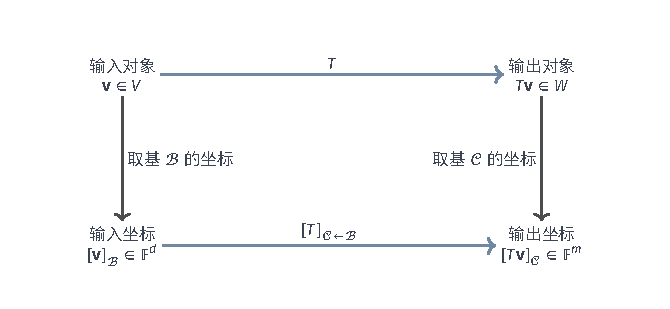
\includegraphics[width=112.0mm]{figures/00-shared/mathematical-preliminaries-upper/02-linear-spaces/tikz/ch06-object-coordinate-map/figure.pdf}
  \caption{先作用于对象再取坐标，与先取输入坐标再按矩阵的列作线性组合（即乘矩阵），得到相同输出坐标。横向箭头改变对象或数值，竖向箭头只改变记录方式。}
  \label{fig:ch06-object-coordinate-map}
\end{figure}

\subsubsection{基于矩阵的映射运算}
\phantomsection
\label{sec:ls-map-addition-composition}

映射之间有几种常用运算：把两个映射的输出相加，让两个映射接连作用，撤销一个映射。在固定基下，它们分别记录为第~\ref{chap:linear-operations}章的矩阵加法、乘法与求逆。带常数偏置的仿射映射不是线性映射，但可以借增广坐标写成一张更大的矩阵。

\paragraph{叠加}
\phantomsection
\label{sec:linear-algebra-map-addition}
设$T,S:V\to W$是同一对空间之间的两个线性映射，定义
\[
(aT+bS)(\bm x)=aT\bm x+bS\bm x,\qquad\bm x\in V,\ a,b\in\mathbb R.
\]

把输入的线性组合代入，两项分别展开再汇总，可知叠加仍是线性映射。在$V$与$W$的固定基下，设$T,S$的矩阵为$\bm A,\bm B$。$aT+bS$把第$j$个基向量送到$aT\bm b_j+bS\bm b_j$，其坐标是$a\bm A_{:,j}+b\bm B_{:,j}$，所以$aT+bS$的矩阵就是$a\bm A+b\bm B$。

相加要求两个映射的定义域相同、陪域也相同，这对应于只有同形矩阵才能相加。它不要求$V=W$：两个从$\mathbb R^2$到$\mathbb R^3$的映射可以相加，但不能与一个从$\mathbb R^3$到$\mathbb R^2$的映射相加。系数$a,b$必须与输入无关；若系数随$\bm x$改变，叠加的结果一般不再线性，需要单独检验。

\paragraph{复合}
设$T:U\to V$、$S:V\to W$是线性映射。复合$S\circ T$先作用$T$、再作用$S$，仍保持线性组合：
\[
 S(T(a\bm x+b\bm y))=S(aT\bm x+bT\bm y)=aS(T\bm x)+bS(T\bm y).
\]
取$U,V,W$的基$\mathcal B,\mathcal C,\mathcal D$。对每个$\bm x\in U$，两次使用式~\eqref{eq:linear-algebra-map-matrix-representation}，再用矩阵乘法的结合律，得
\[
 \begin{aligned}
 [S(T\bm x)]_{\mathcal D}
 &=[S]_{\mathcal D\leftarrow\mathcal C}[T\bm x]_{\mathcal C}\\
 &=[S]_{\mathcal D\leftarrow\mathcal C}\bigl([T]_{\mathcal C\leftarrow\mathcal B}[\bm x]_{\mathcal B}\bigr)\\
 &=\bigl([S]_{\mathcal D\leftarrow\mathcal C}[T]_{\mathcal C\leftarrow\mathcal B}\bigr)[\bm x]_{\mathcal B}.
 \end{aligned}
\]
取$\bm x=\bm b_j$，其坐标是$\bm e_j$，两边读出的是$[S\circ T]_{\mathcal D\leftarrow\mathcal B}$与乘积的第$j$列，所以
\begin{equation}
 [S\circ T]_{\mathcal D\leftarrow\mathcal B}
 =[S]_{\mathcal D\leftarrow\mathcal C}\,[T]_{\mathcal C\leftarrow\mathcal B}.
 \label{eq:ls-composition-matrix}
\end{equation}

复合的矩阵是矩阵的乘积，中间空间$V$的基$\mathcal C$在乘积中消去；第~\ref{sec:prelim-linear-actions-composition}节的推导是这里取标准基的特例。恒等映射$\operatorname{id}_V$在同一组基下的矩阵是单位矩阵。映射复合的结合律对应矩阵乘法的结合律；矩阵乘法不可交换，对应先后作用的次序不能交换。

对算子$T:V\to V$两端都用基$\mathcal B$，反复使用式~\eqref{eq:ls-composition-matrix}，得
\[
 [T^k]_{\mathcal B}=([T]_{\mathcal B})^k .
\]
算子的反复作用因此记录为第~\ref{sec:ls-matrix-power-rules}节的矩阵幂。例如对示例~\ref{ex:ls-derivative-matrix}中的$[D]$直接相乘可得$[D]^3=\bm0$，这对应于任何次数不超过$2$的多项式求导三次都变为零。

\paragraph{逆映射}
第~\ref{sec:prelim-inverse-matrices}节把满足$\bm A\bm B=\bm B\bm A=\bm I$的方阵$\bm A$称为可逆矩阵，那里只把它看成可以撤销的数表运算。有了矩阵表示，可以说明它记录的是哪一类映射。

若线性映射$T:V\to W$是双射，每个输出恰有一个原输入，逆映射$T^{-1}:W\to V$存在。逆映射自动是线性的：对$\bm w,\bm w'\in W$，由$T$的线性性
\[
 T\bigl(aT^{-1}\bm w+bT^{-1}\bm w'\bigr)=a\bm w+b\bm w',
\]
所以$aT^{-1}\bm w+bT^{-1}\bm w'$就是$a\bm w+b\bm w'$唯一的原输入，即
\[
 T^{-1}(a\bm w+b\bm w')=aT^{-1}\bm w+bT^{-1}\bm w'.
\]
这样的$T$称为可逆线性映射。

可逆映射与可逆矩阵相互对应。设$T:V\to W$可逆，在基$\mathcal B,\mathcal C$下$\bm A=[T]_{\mathcal C\leftarrow\mathcal B}$，$\bm B=[T^{-1}]_{\mathcal B\leftarrow\mathcal C}$。由式~\eqref{eq:ls-composition-matrix}，$T^{-1}\circ T=\operatorname{id}_V$与$T\circ T^{-1}=\operatorname{id}_W$分别给出$\bm B\bm A=\bm I$与$\bm A\bm B=\bm I$。所以$\bm A$是可逆方阵（下一小节将说明此时必有$\dim V=\dim W$），且$[T^{-1}]_{\mathcal B\leftarrow\mathcal C}=\bm A^{-1}$。

反过来，若$\bm A$可逆，$\bm y\mapsto\bm A^{-1}\bm y$就是$\bm x\mapsto\bm A\bm x$的逆映射。

两个可逆映射接连作用时，$(S\circ T)^{-1}=T^{-1}\circ S^{-1}$，在矩阵上就是式~\eqref{eq:ls-inverse-product}。判断一个映射是否可逆，要先知道它丢失了什么、能到达什么，这由下一小节处理。

\paragraph{仿射映射}
\phantomsection
\label{sec:ls-affine-maps}
线性模型的预测常带截距，平面上的平移也常与旋转一起出现，这些作用都不把原点留在原处。带常数偏置的规则$\bm x\mapsto\bm A\bm x+\bm b$称为\term{仿射映射}（affine map）。当$\bm b\neq\bm0$时，它把$\bm0$送到$\bm b$，所以不是线性映射；当$\bm b=\bm0$时，它就是线性映射。

两个仿射映射$\bm x\mapsto\bm A_1\bm x+\bm b_1$、$\bm y\mapsto\bm A_2\bm y+\bm b_2$复合，得到
\[
 \bm x\mapsto\bm A_2\bm A_1\bm x+(\bm A_2\bm b_1+\bm b_2),
\]
前一个映射的平移项也受到后一个映射的作用。

给坐标补一个恒为$1$的末位，仿射映射就能写成高一维空间上的线性作用：
\begin{equation}
 \begin{bmatrix}\bm A&\bm b\\ \bm0^\top&1\end{bmatrix}
 \begin{bmatrix}\bm x\\1\end{bmatrix}
 =
 \begin{bmatrix}\bm A\bm x+\bm b\\1\end{bmatrix}.
 \label{eq:ls-affine-homogeneous}
\end{equation}
按分块乘法，两个这样的增广矩阵相乘得
\[
 \begin{bmatrix}\bm A_2&\bm b_2\\ \bm0^\top&1\end{bmatrix}
 \begin{bmatrix}\bm A_1&\bm b_1\\ \bm0^\top&1\end{bmatrix}
 =\begin{bmatrix}\bm A_2\bm A_1&\bm A_2\bm b_1+\bm b_2\\ \bm0^\top&1\end{bmatrix},
\]
正是复合仿射映射的增广矩阵。

增广矩阵在整个增广空间上是线性的，但原输入只取末坐标为$1$的向量，所以不能据此说原映射线性。第~\ref{chap:linear-solution-selection}章用这种形式描述仿射解集的几何。

\subsubsection{矩阵基本子空间}
\phantomsection
\label{sec:ls-four-fundamental-subspaces}

矩阵$\bm A\in\mathbb R^{m\times d}$给出从$\mathbb R^d$到$\mathbb R^m$的映射$\bm x\mapsto\bm A\bm x$，它的转置$\bm A^\top\in\mathbb R^{d\times m}$给出反方向的映射$\bm y\mapsto\bm A^\top\bm y$。对每个方向可以问两个问题：哪些输出能够到达，哪些输入被送到零。四个答案都是子空间，它们刻画了矩阵保留和丢失的信息。

按矩阵与向量乘积的列读法，$\bm A\bm x=\sum_jx_j\bm A_{:,j}$。$\bm x$取遍$\mathbb R^d$时，输出取遍$\bm A$各列的全部线性组合，即各列的张成空间，称为$\bm A$的\term{列空间}（column space），记为$\operatorname{range}(\bm A)$。所以方程$\bm A\bm x=\bm b$有解，当且仅当$\bm b\in\operatorname{range}(\bm A)$。

齐次方程组$\bm A\bm x=\bm0$的解集合是$\mathbb R^d$的子空间（示例~\ref{ex:ls-subspace-checks}），称为$\bm A$的\term{零空间}（null space），记为$\operatorname{null}(\bm A)$。

对$\bm A^\top$问同样的两个问题，又得到两个子空间。$\bm A^\top$的列就是$\bm A$的行，所以$\operatorname{range}(\bm A^\top)$由$\bm A$各行的线性组合组成，称为$\bm A$的\term{行空间}（row space）。

$\bm A^\top\bm y=\bm0$转置后就是$\bm y^\top\bm A=\bm0^\top$，即$\bm y^\top$从左边乘$\bm A$得到零，所以$\operatorname{null}(\bm A^\top)$称为$\bm A$的\term{左零空间}（left null space）。

这四个子空间合称$\bm A$的\term{四个基本子空间}（four fundamental subspaces）：
\begin{equation}
 \begin{aligned}
  \operatorname{range}(\bm A)&=\{\bm A\bm x:\bm x\in\mathbb R^d\}\subseteq\mathbb R^m,\\
  \operatorname{null}(\bm A)&=\{\bm x\in\mathbb R^d:\bm A\bm x=\bm0\}\subseteq\mathbb R^d,\\
  \operatorname{range}(\bm A^\top)&=\{\bm A^\top\bm y:\bm y\in\mathbb R^m\}\subseteq\mathbb R^d,\\
  \operatorname{null}(\bm A^\top)&=\{\bm y\in\mathbb R^m:\bm A^\top\bm y=\bm0\}\subseteq\mathbb R^m.
 \end{aligned}
 \label{eq:ls-four-fundamental-subspaces}
\end{equation}

零空间与行空间在输入空间$\mathbb R^d$中，列空间与左零空间在输出空间$\mathbb R^m$中。零空间收集被完全消去的输入方向。

行空间收集读取输出分量所用的方向：输出的第$i$个分量$(\bm A\bm x)_i=\bm A_{i,:}\bm x$由第$i$行与$\bm x$逐项相乘再相加得到。

左零空间收集对可达输出读数恒为零的加权方式：对$\bm y\in\operatorname{null}(\bm A^\top)$与任意输入$\bm x$，
\[
 \bm y^\top(\bm A\bm x)=(\bm y^\top\bm A)\bm x=0 .
\]

下面对一个具体矩阵求出四个基本子空间。
\begin{example}[一个$2\times3$矩阵的四个基本子空间]
\label{ex:ls-rank-one-four-subspaces}
取
\[
 \bm A=\begin{bmatrix}1&2&3\\2&4&6\end{bmatrix}\in\mathbb R^{2\times3}.
\]
它的第二行是第一行的$2$倍，每一列也都是$(1,2)^\top$的倍数，四个子空间都可以直接读出。

先看输出空间$\mathbb R^2$。三列$(1,2)^\top$、$(2,4)^\top$、$(3,6)^\top$都落在同一条直线上，所以列空间$\operatorname{range}(\bm A)=\operatorname{span}\{(1,2)^\top\}$。左零空间要求
\[
 \bm y^\top\bm A=(y_1+2y_2)(1,2,3)
\]
为零，即$y_1=-2y_2$，所以$\operatorname{null}(\bm A^\top)=\operatorname{span}\{(2,-1)^\top\}$，也是一条直线。

再看输入空间$\mathbb R^3$。两行都是$(1,2,3)$的倍数，所以行空间是一条直线：
\[
 \operatorname{range}(\bm A^\top)=\operatorname{span}\{(1,2,3)^\top\}.
\]
因为第二行重复第一行，$\bm A\bm x=\bm0$只剩一个方程$x_1+2x_2+3x_3=0$，由示例~\ref{ex:ls-solution-plane-basis}，零空间
\[
 \operatorname{null}(\bm A)=\operatorname{span}\{(-2,1,0)^\top,(-3,0,1)^\top\}
\]
是一个平面。

四个维数依次为：列空间$1$、零空间$2$、行空间$1$、左零空间$1$。其中有两条规律。一是列空间与行空间维数相同。二是同一端的两个子空间维数互补。

此外，行空间的方向$(1,2,3)^\top$与零空间的两个基向量逐项相乘再相加都得零，列空间的方向$(1,2)^\top$与左零空间的方向$(2,-1)^\top$也是如此。
\end{example}
第~\ref{sec:ls-kernel-image}节将证明，示例中的两条维数规律对任何矩阵都成立；垂直关系要等第~\ref{sec:ls-orthogonality}节有了内积才能说清。

\subsection{核、像与秩}
\label{sec:ls-kernel-image}

能否由输出反求输入，取决于映射丢失了哪些输入信息、能产生哪些输出。本小节把这两方面写成核与像两个子空间，用秩零度定理联系二者的维数，再从商空间的角度重新解释这一关系，最后算出矩阵四个基本子空间的维数。

\paragraph{核与像}
被映射送到零的输入集合称为$T$的核（kernel），记为
\[
 \ker T=\{\bm x\in V:T\bm x=\bm0\};
\]
所有可到达的输出组成的集合称为\term{像空间}（简称像，image），记为
\[
 \operatorname{im}T=\{T\bm x:\bm x\in V\}.
\]
二者都是子空间：若$T\bm x=T\bm y=\bm0$，则$T(a\bm x+b\bm y)=\bm0$；若$\bm u=T\bm x$、$\bm v=T\bm y$，则$a\bm u+b\bm v=T(a\bm x+b\bm y)$。

核位于输入端，像位于输出端，二者不在同一空间中，不能直接比较。对矩阵$\bm A\in\mathbb R^{m\times d}$，映射$\bm x\mapsto\bm A\bm x$的核就是零空间$\operatorname{null}(\bm A)$，像就是列空间$\operatorname{range}(\bm A)$（第~\ref{sec:ls-four-fundamental-subspaces}节）。说“矩阵$\bm A$的核”“矩阵$\bm A$的秩”时，指的都是映射$\bm x\mapsto\bm A\bm x$的相应量。

核代表丢失的信息，理由如下：$T\bm x=T\bm y$当且仅当$T(\bm x-\bm y)=\bm0$，即$\bm x-\bm y\in\ker T$。所以两个输入相差一个核中的向量时，输出完全相同。下面的例子用三个响应读取四个分量，展示这一点。
\begin{example}[相差核方向的输入给出相同输出]
\label{ex:ls-kernel-indistinguishable}
设$T:\mathbb R^4\to\mathbb R^3$把第四个分量分别加到前三个分量上：
\[
 T(x_1,x_2,x_3,x_4)=(x_1+x_4,\ x_2+x_4,\ x_3+x_4).
\]
三个响应全为零，要求$x_1=x_2=x_3=-x_4$，所以$\ker T=\operatorname{span}\{(1,1,1,-1)^{\top}\}$。

另一方面，取$x_4=0$时$T\bm x=(x_1,x_2,x_3)$可以是任意向量，所以$\operatorname{im}T=\mathbb R^3$：每个输出都能到达，但核不为零。

具体比较两个输入$(1,1,1,1)^\top$与$(0,0,0,2)^\top$。它们之差$(1,1,1,-1)^\top$恰在核中，于是
\[
 T(1,1,1,1)=T(0,0,0,2)=(2,2,2).
\]
仅凭三个响应无法区分这两个输入；同样的论证说明，任何两个相差$(1,1,1,-1)^\top$倍数的输入都无法区分。
\end{example}
这就是线性不可辨识性：两个输入相差核方向时输出相同，只凭输出无法确定输入。若另有约束限制了可取的输入，能否辨识还要结合这些约束判断。

\paragraph{秩零度定理}
\phantomsection
\label{sec:ls-rank-nullity}
核与像的维数之间有一个精确的关系。像的维数称为\term{秩}（rank），记为$\operatorname{rank}T=\dim\operatorname{im}T$；核的维数称为\term{零度}（nullity），即$\dim\ker T$。
\begin{theorem}[秩零度定理]
\label{thm:ls-rank-nullity}
\label{thm:linear-algebra-rank-nullity}
有限维线性映射$T:V\to W$满足
\begin{equation}
\begin{gathered}
\dim V=\dim\ker T+\dim\operatorname{im}T\\
\text{即}\qquad
 \dim V=\dim\ker T+\operatorname{rank}T.
\end{gathered}
\label{eq:ls-rank-nullity}
\end{equation}
\end{theorem}
\begin{proof}
取核的一组基$\bm v_1,\ldots,\bm v_r$，扩充成$V$的基$\bm v_1,\ldots,\bm v_d$。前$r$个基向量的像为零，所以其余的像$T\bm v_{r+1},\ldots,T\bm v_d$张成像。若$\sum_{j>r}a_jT\bm v_j=\bm0$，则$\sum_{j>r}a_j\bm v_j$属于核，能由前$r$个基向量表示；整组基的线性无关性迫使全部$a_j=0$，所以这些像线性无关。于是像的维数为$d-r$，结论成立。
\end{proof}
对矩阵$\bm A\in\mathbb R^{m\times d}$，记$\operatorname{rank}\bm A$为其映射的秩，即列空间的维数，则
\[
 d=\dim\operatorname{null}(\bm A)+\operatorname{rank}\bm A.
\]
秩计数独立的输出方向，零度计数被消去的独立输入方向，二者之和固定为输入维数。在示例~\ref{ex:ls-kernel-indistinguishable}中，$\dim\ker T=1$、$\operatorname{rank}T=3$，二者之和为输入维数$4$。图~\ref{fig:ls-kernel-image-rank-nullity}再给出两个几何算例：被送到零的方向与实际用到的输出方向，维数相加恰为定义域的维数。
\begin{figure*}[htbp]
  \centering
  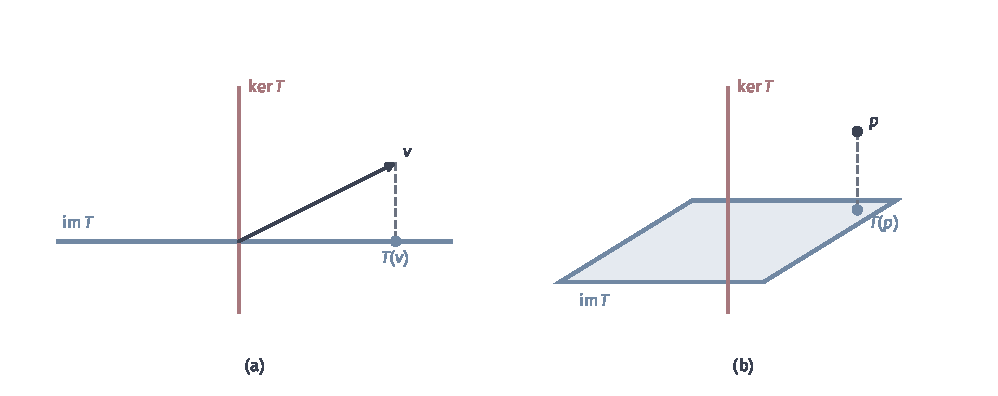
\includegraphics[width=169mm]{figures/00-shared/mathematical-preliminaries-upper/02-linear-spaces/matplotlib/ls-kernel-image-rank-nullity/ls-kernel-image-rank-nullity.pdf}
  \caption{核与像的维数此消彼长。两幅共用图面基线，红色表示核，蓝色表示像。(a)~$T(x,y)=(x,0)$把平面映到$x$轴，$\bm v=(2,1)$被映到$(2,0)$，核与像各为一维，$1+1=2$。(b)~$T(x,y,z)=(x,y)$的核是$z$轴，像是二维平面，$1+2=3$；斜投影图中$\bm p=(1,1,1)$沿虚线落到$T(\bm p)=(1,1)$。平面画在输入空间的$xy$位置，用来表示输出的两个坐标。}
  \label{fig:ls-kernel-image-rank-nullity}
\end{figure*}

秩不超过矩阵的行数和列数：$\operatorname{rank}\bm A\leq\min(m,d)$。这是因为列空间在$\mathbb R^m$中，维数不超过$m$；它又由$d$列张成，从中抽取的基不超过$d$个向量。$\operatorname{rank}\bm A=d$称为满列秩，这时输入方向全部保留，等价于各列线性无关；$\operatorname{rank}\bm A=m$称为满行秩，这时每个输出都可以到达。二者统称\term{满秩}（full rank）。

矩形矩阵不能同时满列秩和满行秩。$m<d$时，即使满行秩，核的维数也是$d-m>0$；$m>d$时，即使满列秩，像的维数也只有$d<m$，总有输出无法到达。

例如贯穿例$\bm X_\varepsilon$在$\varepsilon\neq0$时两列线性无关（示例~\ref{ex:ls-nearly-collinear-independence}），秩为$2$，满列秩；它的像是$\mathbb R^3$中的一个平面，所以不是满行秩。

\paragraph{商空间}
前面看到，输出相同的输入恰好彼此相差一个核中的向量。按输出把输入分组，每组都形如$\bm x+\ker T$，正是第~\ref{sec:ls-quotient-spaces}节取$U=\ker T$得到的等价类；全部分组组成商空间$V/\ker T$。

规则$\bm x+\ker T\mapsto T\bm x$不依赖代表元，因为代表元相差核中的向量时输出相同。它保持线性组合，并且满射到$\operatorname{im}T$。它也是单射：两个类的像相同即$T\bm x=T\bm y$时，$\bm x-\bm y\in\ker T$，两个类相同。所以它是从$V/\ker T$到$\operatorname{im}T$的线性双射。压去全部丢失的方向以后，每个等价类恰好对应一个可达输出。

线性双射把一组基送到一组基，所以两边维数相同。由式~\eqref{eq:ls-quotient-dimension}得
\[
 \dim V-\dim\ker T=\operatorname{rank}T,
\]
这是秩零度定理的另一种读法。在示例~\ref{ex:ls-kernel-indistinguishable}中，商空间$\mathbb R^4/\ker T$是三维的，像$\mathbb R^3$也是三维的。

\paragraph{证明行秩等于列秩}
现在对一般的$\bm A\in\mathbb R^{m\times d}$证明示例~\ref{ex:ls-rank-one-four-subspaces}中的维数规律。对$\bm A$用秩零度定理，零空间与列空间的维数之和为$d$；对$\bm A^\top$用秩零度定理，左零空间与行空间的维数之和为$m$。还需证明行空间与列空间的维数总相等。
\begin{theorem}[行秩等于列秩]
\label{thm:ls-row-rank-column-rank}
对任意$\bm A\in\mathbb R^{m\times d}$，$\dim\operatorname{range}(\bm A^\top)=\dim\operatorname{range}(\bm A)$，即$\operatorname{rank}\bm A^\top=\operatorname{rank}\bm A$。
\end{theorem}
\begin{proof}
设$r=\operatorname{rank}\bm A$，取列空间的一组基$\bm c_1,\ldots,\bm c_r$，排成$\bm C\in\mathbb R^{m\times r}$。$\bm A$的每一列都在列空间中，所以第$j$列可写成$\bm A_{:,j}=\bm C\bm r_j$，$\bm r_j\in\mathbb R^r$；把这些系数列排成$\bm R\in\mathbb R^{r\times d}$，按乘积的列读法得
\[
 \bm A=\bm C\bm R .
\]

再按行读这个乘积：$\bm A$的第$i$行是
\[
 \bm A_{i,:}=\sum_{k=1}^r\bm C_{i,k}\bm R_{k,:},
\]
即$\bm R$的$r$行的线性组合。所以$\bm A$的全部行都落在$\bm R$的$r$行张成的空间里，行空间的维数不超过$r$，即$\operatorname{rank}\bm A^\top\leq\operatorname{rank}\bm A$。对$\bm A^\top$用同样的论证，得$\operatorname{rank}\bm A\leq\operatorname{rank}\bm A^\top$，两者相等。
\end{proof}
于是行秩（行空间的维数）与列秩（列空间的维数）可以统称为秩。对$\bm A$与$\bm A^\top$分别用秩零度定理，四个基本子空间的维数全部由$m,d$与$r=\operatorname{rank}\bm A$决定：
\begin{equation}
 \begin{gathered}
 \dim\operatorname{range}(\bm A)=\dim\operatorname{range}(\bm A^\top)=r,\\
 \dim\operatorname{null}(\bm A)=d-r,\qquad
 \dim\operatorname{null}(\bm A^\top)=m-r.
 \end{gathered}
 \label{eq:ls-four-subspace-dimensions}
\end{equation}
输入空间中的零空间与行空间维数相加为$d$，输出空间中的列空间与左零空间维数相加为$m$。

对示例~\ref{ex:ls-rank-one-four-subspaces}中的$\bm A$，$r=1$，式~\eqref{eq:ls-four-subspace-dimensions}给出的维数与直接计算一致；证明中的分解$\bm A=\bm C\bm R$在那里就是
\[
 \bm A=(1,2)^\top(1,2,3).
\]
该示例还显示，两对子空间不仅维数互补，而且互相垂直，这要等第~\ref{sec:ls-orthogonality}节有了内积才能说清。第~\ref{sec:ls-dual-map}节还将用对偶映射给出行秩等于列秩的另一个证明。

\subsection{单射、满射与可逆性}
\phantomsection
\label{sec:ls-injective-surjective-invertible}
线性映射$T:V\to W$可逆，是说每个输出都能唯一地还原出输入。这包含两个要求：不同的输入不会给出相同的输出，称为单射；输出空间中的每个向量都能被某个输入到达，称为满射。两者都成立时称为双射，也就是可逆。对线性映射，这两个要求都可以用上一小节的核与像来检验。

\paragraph{单射与核}
单射当且仅当核为零。原因是$T\bm x=T\bm y$等价于$T(\bm x-\bm y)=\bm0$，即$\bm x-\bm y\in\ker T$。若核只含零向量，输出相同就迫使输入相同；反过来，若核中有非零向量$\bm z$，它与$\bm0$给出相同的输出$\bm0$，映射就不是单射。

\paragraph{满射与像}
满射按定义就是像等于整个输出空间。在有限维情形，两条判据都可以换成秩的条件。由秩零度定理$\dim\ker T=\dim V-\operatorname{rank}T$，核为零等价于$\operatorname{rank}T=\dim V$；像是$W$的子空间，它等于$W$当且仅当$\operatorname{rank}T=\dim W$。所以
\[
 T\text{单射}\iff\operatorname{rank}T=\dim V,\qquad
 T\text{满射}\iff\operatorname{rank}T=\dim W.
\]

\paragraph{维数与可逆性}
秩至多等于两端维数中较小的一个，所以两端维数的关系先决定了哪些性质可能成立。

若$\dim V<\dim W$，像的维数至多为$\dim V$，映射不可能满射；若$\dim V>\dim W$，核的维数至少为$\dim V-\dim W>0$，映射不可能单射。

因此，只有输入与输出维数相等的映射才可能可逆；矩形矩阵即使满秩，也只能是单射或满射之一。

维数相等时，情况反而简单。$\dim V=\dim W$时上面两个秩条件是同一个条件，单射、满射与可逆互相等价，只需检查其中任意一条，例如核是否为零。

\paragraph{方阵的可逆判据}
把这些结论用到$n$阶方阵$\bm A$上，再结合上一小节可逆映射与逆矩阵的对应，得到一串等价条件：
\[
 \bm A\text{可逆}
 \iff\operatorname{null}(\bm A)=\{\bm0\}
 \iff\operatorname{rank}\bm A=n
 \iff\bm A\text{的}n\text{列线性无关}.
\]
最后一步成立，是因为列空间由$n$列张成，维数为$n$恰好说明这$n$列构成它的一组基。由行秩等于列秩，还可以在链中加入“$\bm A$的$n$行线性无关”。

下面两个矩阵都用同一个判据检验：方阵的核是否为零。
\begin{example}[用核判断可逆]
\label{ex:ls-kernel-invertibility}
对角矩阵$\operatorname{diag}(d_1,\ldots,d_n)$逐坐标缩放，坐标之间互不影响。若每个$d_i\neq0$，逐坐标除以$d_i$即可撤销，逆矩阵为$\operatorname{diag}(1/d_1,\ldots,1/d_n)$。若某个$d_i=0$，$\bm e_i$就落入核中：两个只在第$i$个坐标上不同的输入给出相同的输出，无法还原。所以对角矩阵可逆当且仅当全部$d_i\neq0$。

矩阵
\[
 \bm A=\begin{bmatrix}2&1\\0&3\end{bmatrix}
\]
把两个坐标掺在一起，不能逐坐标撤销，但判据照样适用。$\bm A\bm x=\bm0$即
\[
 2x_1+x_2=0,\qquad 3x_2=0 .
\]
第二式给出$x_2=0$，代入第一式得$x_1=0$。核为零，所以$\bm A$可逆；按第~\ref{sec:prelim-inverse-matrices}节的二阶公式，
\[
 \bm A^{-1}=\frac16\begin{bmatrix}3&-1\\0&2\end{bmatrix}.
\]
\end{example}

这条判据不借助行列式，就能推出关于方阵的两个常用结论。

第一，方阵的单侧逆就是逆（第~\ref{sec:ls-square-one-sided-inverse}节曾用行列式证明）。若$n$阶方阵满足$\bm B\bm A=\bm I_n$，则$\bm A\bm x=\bm0$蕴含
\[
 \bm x=\bm B\bm A\bm x=\bm0,
\]
核为零，所以$\bm A$可逆，进而
\[
 \bm B=\bm B\bm A\bm A^{-1}=\bm A^{-1};
\]$\bm A\bm B=\bm I_n$时对$\bm B$作同样论证。

第二，若$n$阶方阵的乘积$\bm A\bm B$可逆，则两个因子都可逆。$\bm B\bm x=\bm0$蕴含$\bm A\bm B\bm x=\bm0$，从而$\bm x=\bm0$，所以$\bm B$的核为零、$\bm B$可逆；于是$\bm A=(\bm A\bm B)\bm B^{-1}$是两个可逆矩阵的乘积，也可逆。

\paragraph{单侧逆}
维数不同时不能完全撤销，但可以从一侧撤销。若$T:V\to W$是单射，存在线性映射$L:W\to V$使$L\circ T=\operatorname{id}_V$：在像上按$T$的逆读回输入，在像的一个补空间上任意规定，例如全部送到零。若$T$是满射，存在线性映射$R:W\to V$使$T\circ R=\operatorname{id}_W$：为输出基中的每个向量任选一个原像，再线性延拓。补空间与原像都有多种选法，所以这些单侧逆一般不唯一。

写成矩阵，对$\bm A\in\mathbb R^{m\times d}$：$\bm A$有左逆当且仅当它满列秩，有右逆当且仅当它满行秩。充分性来自上面的构造，因为满列秩就是单射，满行秩就是满射。必要性同样直接：若$\bm L\bm A=\bm I_d$，则$\bm A\bm x=\bm0$蕴含$\bm x=\bm L\bm A\bm x=\bm0$，核为零；若$\bm A\bm R=\bm I_m$，则每个$\bm y=\bm A(\bm R\bm y)$都能到达。

\subsection{换基与相抵}
\label{sec:ls-coordinates-change-of-basis}
\phantomsection
\label{sec:ls-equivalence-matrices}

第~\ref{sec:ls-coordinates}节看到，同一个向量在不同的基下有不同的坐标。线性映射也是这样：映射本身不变，换一组基，记录它的矩阵通常就会改变。这一小节和下一小节写出这种变化的规律，并回答一个反方向的问题：给定两个矩阵，怎样判断它们记录的是不是同一个映射。

需要区分两种情形。一般的线性映射$T:V\to W$两端是两个空间，可以各自换基，由此得到的矩阵关系称为相抵，是本小节的内容。线性算子$T:V\to V$两端是同一个空间，换基时两端必须一起换，由此得到的关系称为相似，留到下一小节。相似多了“两端换基相同”这一约束，可调整的余地更小：后面会看到，相抵只用秩就能完全分类，相似则需要更多不变量。

推导时要用到一个观察：换基矩阵本身就是一个线性映射的矩阵。比较式~\eqref{eq:linear-algebra-coordinate-change}与式~\eqref{eq:linear-algebra-map-matrix-representation}可见，$\bm S_{\mathcal C\leftarrow\mathcal B}$正是恒等映射$\operatorname{id}_V$以$\mathcal B$为输入基、$\mathcal C$为输出基的矩阵：向量不动，只是两端用不同的基记录。连续换基时换基矩阵相乘，就是复合公式~\eqref{eq:ls-composition-matrix}用于$\operatorname{id}_V\circ\operatorname{id}_V=\operatorname{id}_V$的特例。

下面设$T:V\to W$是线性映射，$\dim V=d$、$\dim W=m$。先求出$T$在两对基下的矩阵之间的关系，再说明这一关系恰好刻画“记录同一个映射”，最后证明只需比较秩就能判断。

\subsubsection{相抵的定义}
\label{sec:ls-equivalence-definition}
先从换基推导两种记录之间的关系，再据此给出定义。

设$\mathcal B,\mathcal B'$是$V$的旧基与新基，$\mathcal C,\mathcal C'$是$W$的旧基与新基，$T$在旧基下的矩阵为$\bm A=[T]_{\mathcal C\leftarrow\mathcal B}$，在新基下的矩阵为$\bm B=[T]_{\mathcal C'\leftarrow\mathcal B'}$。两端的换基矩阵记为
\[
 \bm P=\bm S_{\mathcal B\leftarrow\mathcal B'}\ (d\text{阶可逆}),\qquad
 \bm Q=\bm S_{\mathcal C\leftarrow\mathcal C'}\ (m\text{阶可逆}),
\]
$\bm P$的第$j$列是第$j$个新输入基向量在旧输入基下的坐标，$\bm Q$同理。

要从新输入坐标$[\bm v]_{\mathcal B'}$求出新输出坐标$[T\bm v]_{\mathcal C'}$，可以绕道旧基走三步。先把新输入坐标换成旧输入坐标，再在旧基下作用：
\[
 [\bm v]_{\mathcal B}=\bm P[\bm v]_{\mathcal B'},\qquad
 [T\bm v]_{\mathcal C}=\bm A[\bm v]_{\mathcal B}.
\]
最后用反向换基矩阵$\bm Q^{-1}=\bm S_{\mathcal C'\leftarrow\mathcal C}$把旧输出坐标换成新输出坐标。合起来是
\[
 [T\bm v]_{\mathcal C'}=\bm Q^{-1}[T\bm v]_{\mathcal C}=\bm Q^{-1}\bm A\bm P[\bm v]_{\mathcal B'}.
\]

另一方面，按定义
\[
 [T\bm v]_{\mathcal C'}=\bm B[\bm v]_{\mathcal B'} .
\]
两式对每个$\bm v$都成立。取$\bm v$为第$j$个新输入基向量，它的新坐标是$\bm e_j$，两边读出的就是两个矩阵的第$j$列。所以
\begin{equation}
 \bm B=\bm Q^{-1}\bm A\bm P.
 \label{eq:ls-equivalence-transform}
\end{equation}
从右向左读，$\bm P$把新输入坐标换成旧坐标，$\bm A$在旧基下作用，$\bm Q^{-1}$把结果换成新输出坐标。也可以用复合来理解：$T=\operatorname{id}_W\circ T\circ\operatorname{id}_V$，三个因子各自在相应的基下记录，由式~\eqref{eq:ls-composition-matrix}就得到右端的三个矩阵。

\phantomsection
\label{sec:ls-equivalence-meaning}%
上面的推导表明，同一个映射的两种记录之间，只差在两侧各乘一个可逆矩阵。把这种关系单独命名。
\begin{definition}[矩阵相抵]
\label{def:ls-matrix-equivalence}
设$\bm A,\bm B\in\mathbb R^{m\times d}$。若存在可逆矩阵$\bm Q\in\mathbb R^{m\times m}$与$\bm P\in\mathbb R^{d\times d}$使$\bm B=\bm Q^{-1}\bm A\bm P$，就称$\bm A$与$\bm B$\term{相抵}（equivalent matrices）。
\end{definition}
定义中的$\bm Q,\bm P$可以是任意可逆矩阵，不必事先知道它们来自哪组基。写成$\bm Q^{-1}$只是为了与换基推导一致；$\bm Q$取遍全部可逆矩阵时，$\bm Q^{-1}$也取遍全部可逆矩阵。

反过来，任意一对可逆矩阵都对应一次换基，所以相抵恰好刻画“记录同一个映射”。设$\bm A=[T]_{\mathcal C\leftarrow\mathcal B}$，任给可逆的$\bm P,\bm Q$。由第~\ref{sec:ls-coordinates}节，以$\bm P$的各列为旧基下的坐标，可以构造$V$的一组新基$\mathcal B'$，使$\bm S_{\mathcal B\leftarrow\mathcal B'}=\bm P$；输出端用$\bm Q$同样构造$\mathcal C'$。按换基过程，$T$在这两组新基下的矩阵正是$\bm Q^{-1}\bm A\bm P$。因此，两个同形矩阵相抵，当且仅当它们是同一个线性映射在两端不同选基下的记录。

在这个意义下，右乘$\bm P$对应更换输入基，左乘$\bm Q^{-1}$对应更换输出基。初等列变换与初等行变换就是这两种换基最简单的具体形式。

\subsubsection{相抵的性质}
\label{sec:ls-equivalence-properties}
相抵的矩阵记录同一个映射，映射本身的性质就不应随基改变。下面逐条给出相抵的性质。

首先，“相抵”可以像“相等”一样使用：它是等价关系。
\begin{theorem}[相抵是等价关系]
\label{thm:ls-equivalence-relation}
在$\mathbb R^{m\times d}$上：每个矩阵与自身相抵；若$\bm A$与$\bm B$相抵，则$\bm B$与$\bm A$相抵；若$\bm A$与$\bm B$相抵、$\bm B$与$\bm C$相抵，则$\bm A$与$\bm C$相抵。
\end{theorem}
\begin{proof}
自反性取$\bm Q=\bm P=\bm I$。

对称性：由$\bm B=\bm Q^{-1}\bm A\bm P$得$\bm A=\bm Q\bm B\bm P^{-1}=(\bm Q^{-1})^{-1}\bm B\bm P^{-1}$。

传递性：若$\bm B=\bm Q_1^{-1}\bm A\bm P_1$、$\bm C=\bm Q_2^{-1}\bm B\bm P_2$，则$\bm C=(\bm Q_1\bm Q_2)^{-1}\bm A(\bm P_1\bm P_2)$。

三条分别对应不换基、换回原基和连续换两次基。
\end{proof}

其次，换基只是把零空间和列空间“搬”到新的坐标下，并不改变它们。
\begin{theorem}[相抵下的零空间与列空间]
\label{thm:ls-equivalence-subspaces}
若$\bm B=\bm Q^{-1}\bm A\bm P$，其中$\bm Q,\bm P$可逆，则
\[
 \operatorname{null}(\bm B)=\bm P^{-1}\operatorname{null}(\bm A),\qquad
 \operatorname{range}(\bm B)=\bm Q^{-1}\operatorname{range}(\bm A).
\]
\end{theorem}
\begin{proof}
$\bm B\bm x=\bm0$当且仅当$\bm A(\bm P\bm x)=\bm0$，即$\bm P\bm x\in\operatorname{null}(\bm A)$，所以零空间在输入端被$\bm P^{-1}$搬运。又$\bm B\bm x=\bm Q^{-1}\bm A(\bm P\bm x)$，而$\bm x$取遍全部输入时$\bm P\bm x$也取遍全部输入，所以列空间在输出端被$\bm Q^{-1}$搬运。
\end{proof}

最后，可逆矩阵把线性无关组送到线性无关组，因而不改变子空间的维数。由上一定理立即得到最常用的不变量。
\begin{theorem}[相抵保持秩]
\label{thm:ls-equivalence-invariants}
相抵的矩阵$\bm A,\bm B\in\mathbb R^{m\times d}$秩相同，零空间维数也相同：
\begin{equation}
\begin{gathered}
\operatorname{rank}\bm B=\operatorname{rank}\bm A\\
\dim\operatorname{null}(\bm B)=\dim\operatorname{null}(\bm A)=d-\operatorname{rank}\bm A.
\end{gathered}
\label{eq:ls-equivalence-invariants}
\end{equation}
\end{theorem}
\begin{proof}
由定理~\ref{thm:ls-equivalence-subspaces}，$\operatorname{range}(\bm B)$与$\operatorname{null}(\bm B)$分别是$\operatorname{range}(\bm A)$与$\operatorname{null}(\bm A)$在可逆矩阵下的像，维数不变；第二个等式的右端由秩零度定理给出。
\end{proof}

幂、迹这类量不在相抵的讨论之列：相抵允许输入与输出是不同的空间，$\bm B$一般不是方阵，不能对自身反复作用。

\subsubsection{相抵的判据}
\label{sec:ls-equivalence-conditions}
秩在相抵下不变；反过来，秩相同的两个同形矩阵也一定相抵。证明的思路是：两端可以各自选基时，每个矩阵都能化成只由秩决定的简单形状。

设$\bm A$是$T$在某对基下的矩阵，$r=\operatorname{rank}\bm A$。在输入端，取$\ker T$的一组基，再扩充为$V$的一组基；由秩零度定理，新增的向量恰有$r$个，把它们排在前面。这$r$个向量的像线性无关：若像的某个组合为零，相应的新增向量组合就落进核里，能由核的基表示，而整组基线性无关，迫使系数全为零。核的基向量的像都是零，所以这$r$个像还张成$\operatorname{im}T$。

在输出端，把这$r$个像扩充为$W$的一组基。在这样选取的两组基下，$T$把前$r$个输入基向量依次送到前$r$个输出基向量，把其余输入基向量送到零，矩阵为秩标准形
\begin{equation}
 \begin{bmatrix}\bm I_r&\bm0\\\bm0&\bm0\end{bmatrix},\qquad r=\operatorname{rank}\bm A.
\label{eq:ls-rank-normal-form}
\end{equation}

下面对一个秩为$1$的二阶矩阵具体做出这两组基。
\begin{example}[两端各自选基化为秩标准形]
\label{ex:ls-rank-normal-form-two-by-two}
设$T\bm x=\bm A\bm x$，其中
\[
 \bm A=\begin{bmatrix}1&2\\2&4\end{bmatrix},
\]
两端原来都用标准基。两列共线，$\operatorname{rank}\bm A=1$；又$\bm A(-2,1)^\top=\bm0$，所以$\ker T=\operatorname{span}\{(-2,1)^\top\}$。

按上面的构造选基。输入端把核的基向量$\bm v_2=(-2,1)^{\top}$放在后面，前面补一个不在核中的$\bm v_1=\bm e_1$；输出端先取它的像$\bm w_1=\bm A\bm v_1=(1,2)^{\top}$，再补上$\bm w_2=\bm e_2$凑成一组基。以新基向量的标准坐标为列，得到两端的换基矩阵
\[
 \bm P=\begin{bmatrix}1&-2\\0&1\end{bmatrix},\qquad
 \bm Q=\begin{bmatrix}1&0\\2&1\end{bmatrix}.
\]
输出端的换基矩阵还要求逆，得
\[
 \bm Q^{-1}=\begin{bmatrix}1&0\\-2&1\end{bmatrix}.
\]
先算$\bm A\bm P$，它的两列就是$\bm v_1,\bm v_2$的像的标准坐标：
\[
 \bm A\bm P=\begin{bmatrix}1&0\\2&0\end{bmatrix}.
\]
再左乘$\bm Q^{-1}$，把这两个像改用输出基$\bm w_1,\bm w_2$记录：
\[
 \bm Q^{-1}\bm A\bm P=\begin{bmatrix}1&0\\-2&1\end{bmatrix}\begin{bmatrix}1&0\\2&0\end{bmatrix}
 =\begin{bmatrix}1&0\\0&0\end{bmatrix}.
\]
结果正是秩标准形$\operatorname{diag}(1,0)$：在新基下，$T$把$\bm v_1$送到$\bm w_1$，把核方向$\bm v_2$送到零。
\end{example}
图~\ref{fig:ls-equivalence-two-sided-bases-flow}画出这两组基：$\bm v_1$被送到$\bm w_1$，核方向$\bm v_2$被送到零，输出端的$\bm w_2$不被任何输入到达。这几点要同时做到，需要两端各自选基；若要求两端用同一组基，这样的化简一般做不到。
\begin{figure}[!htb]
  \centering
  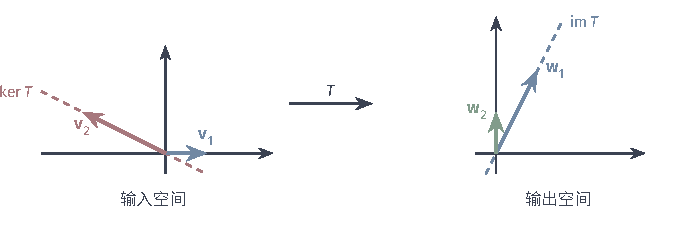
\includegraphics[width=112mm]{figures/00-shared/mathematical-preliminaries-upper/02-linear-spaces/tikz/comprehension-additions/equivalence-two-bases.pdf}
  \caption{两端各自选基化为秩标准形。$T(\bm x)=\bm A\bm x$，$\bm A=\left[\begin{smallmatrix}1&2\\2&4\end{smallmatrix}\right]$。左：输入基$\bm v_1=\bm e_1$（蓝）与$\bm v_2=(-2,1)^{\top}$（红），$\bm v_2$在核（红虚线）上。右：输出基$\bm w_1=T\bm v_1=(1,2)^{\top}$（蓝）位于像（蓝虚线）上，$\bm w_2=\bm e_2$（绿）补足一组基。在这两组基下$T$的矩阵为$\operatorname{diag}(1,0)$。}
  \label{fig:ls-equivalence-two-sided-bases-flow}
\end{figure}

有了秩标准形，就得到相抵的完整判据。
\begin{theorem}[相抵判据]
\label{thm:ls-equivalence-criterion}
两个同形实矩阵$\bm A,\bm B\in\mathbb R^{m\times d}$相抵，当且仅当$\operatorname{rank}\bm A=\operatorname{rank}\bm B$。
\end{theorem}
\begin{proof}
必要性由定理~\ref{thm:ls-equivalence-invariants}得到。充分性：设二者秩都为$r$，由上面的构造，存在可逆矩阵使
\[
 \bm R=\bm Q_A^{-1}\bm A\bm P_A=\bm Q_B^{-1}\bm B\bm P_B,
\]
其中$\bm R$是式\eqref{eq:ls-rank-normal-form}的秩标准形。两式对接得
\[
 \bm B=(\bm Q_A\bm Q_B^{-1})^{-1}\bm A(\bm P_A\bm P_B^{-1}),
\]
即二者相抵。
\end{proof}
所以形状固定以后，秩就是判断相抵的唯一依据：零矩阵只与零矩阵相抵，同形的满秩矩阵彼此相抵。

实际把矩阵化到秩标准形，可以交替使用第~\ref{sec:ls-elementary-row-operations}节的初等行变换与相应的初等列变换；数值计算中的消元算法在第~\ref{chap:direct-linear-solvers}章建立。

\subsection{换基与相似}
\label{sec:ls-similarity}
\phantomsection
\label{sec:ls-matrix-equivalences}

线性算子$T:V\to V$的输入与输出是同一个空间。记录它时两端用同一组基，换基时两端也要换成同一组新基。本小节把这一约束加进上一小节的推导，得到相似关系，再讨论相似保持哪些量，以及怎样判断两个方阵是否相似。

\subsubsection{相似的定义}
\label{sec:ls-similarity-definition}
设$\mathcal B$与$\mathcal B'$是$V$的旧基与新基，$\bm A=[T]_{\mathcal B}$、$\bm B=[T]_{\mathcal B'}$，换基矩阵$\bm P=\bm S_{\mathcal B\leftarrow\mathcal B'}$的第$j$列是第$j$个新基向量在旧基下的坐标。

两端是同一个空间、同一次换基，所以上一小节三步推导中的$\bm Q$就是$\bm P$。先把新坐标换成旧坐标，再在旧基下作用：
\[
 [\bm v]_{\mathcal B}=\bm P[\bm v]_{\mathcal B'},\qquad
 [T\bm v]_{\mathcal B}=\bm A\bm P[\bm v]_{\mathcal B'}.
\]
再把输出换回新坐标，
\[
 [T\bm v]_{\mathcal B'}=\bm P^{-1}[T\bm v]_{\mathcal B}=\bm P^{-1}\bm A\bm P[\bm v]_{\mathcal B'}.
\]
与$[T\bm v]_{\mathcal B'}=\bm B[\bm v]_{\mathcal B'}$逐列比较，得到
\begin{equation}
 \bm B=\bm P^{-1}\bm A\bm P.
 \label{eq:linear-algebra-similarity-change-basis}
\end{equation}
它就是式~\eqref{eq:ls-equivalence-transform}取$\bm Q=\bm P$的情形。

\phantomsection
\label{sec:ls-similarity-meaning}%
与相抵一样，给同一算子两种记录之间的关系单独命名。
\begin{definition}[矩阵相似]
\label{def:ls-matrix-similarity}
设$\bm A,\bm B$是$n$阶方阵。若存在$n$阶可逆矩阵$\bm P$使$\bm B=\bm P^{-1}\bm A\bm P$，就称$\bm A$与$\bm B$\term{相似}（similar）。
\end{definition}
和相抵的论证相同，任意可逆的$\bm P$都对应一次换基：给定$\bm A=[T]_{\mathcal B}$，以$\bm P$的各列为旧基下的坐标构造新基，$T$在新基下的矩阵恰为$\bm P^{-1}\bm A\bm P$。所以两个方阵相似，当且仅当它们是同一个线性算子在两组基下的记录。

注意相似并不要求$\bm A,\bm B$本身可逆，要求可逆的只是换基矩阵$\bm P$。取$\bm Q=\bm P$可见，相似的矩阵一定相抵；反之不然，后面的示例~\ref{ex:ls-equivalent-not-similar}给出秩相同、因而相抵，却不相似的两个矩阵。

换基的一个用处是简化算子的矩阵。下面的例子把一个上三角矩阵化成对角形。
\begin{example}[换基把算子的矩阵化为对角形]
\label{ex:ls-similarity-diagonal}
示例~\ref{ex:ls-plane-operator-matrix}中的算子$T(x_1,x_2)=(2x_1+x_2,3x_2)$在标准基下的矩阵为
\[
 \bm A=\begin{bmatrix}2&1\\0&3\end{bmatrix},
\]
即$T\bm e_1=2\bm e_1$、$T\bm e_2=\bm e_1+3\bm e_2$。$\bm e_1$只被伸长，$\bm e_2$的像却混入了$\bm e_1$方向，这就是非对角元$1$的来源。改取新基$\bm b_1'=\bm e_1$、$\bm b_2'=\bm e_1+\bm e_2$，换基矩阵以新基向量的标准坐标为列，它和它的逆为
\[
 \bm P=\begin{bmatrix}1&1\\0&1\end{bmatrix},\quad
 \bm P^{-1}=\begin{bmatrix}1&-1\\0&1\end{bmatrix},
\]
于是
\[
 \bm B=\bm P^{-1}\bm A\bm P
 =\begin{bmatrix}1&-1\\0&1\end{bmatrix}
 \begin{bmatrix}2&1\\0&3\end{bmatrix}
 \begin{bmatrix}1&1\\0&1\end{bmatrix}.
\]
依次相乘，得
\[
 \bm B=\begin{bmatrix}2&0\\0&3\end{bmatrix}.
\]

不经矩阵乘法也能看出这一结果：$T\bm b_1'=2\bm b_1'$，而
\[
 T\bm b_2'=T\bm e_1+T\bm e_2=3\bm e_1+3\bm e_2=3\bm b_2'.
\]
两个新基方向在$T$的作用下都只被伸缩、不被转向，彼此互不干扰，所以$T$在新基下的矩阵是对角矩阵$\operatorname{diag}(2,3)$。
\end{example}
$T$本身没有改变，改变的只是沿哪两个方向读取它的作用。图~\ref{fig:ls-similarity-change-of-basis-flow}把这一点画在平面上。在标准基下，单位正方形被$T$拉成一个斜的平行四边形，所以矩阵$\bm A$有非零的非对角元；在新基下，基向量围成的平行四边形只沿两个基方向分别伸长$2$倍和$3$倍，所以矩阵是对角的$\bm B$。

\begin{figure}[!htb]
  \centering
  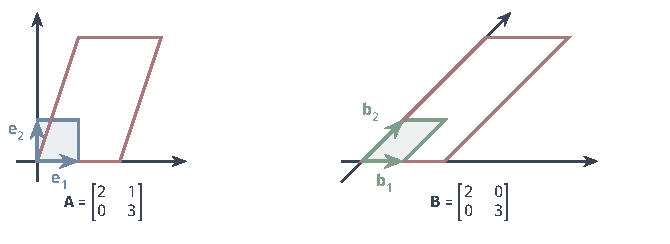
\includegraphics[width=112mm]{figures/00-shared/mathematical-preliminaries-upper/02-linear-spaces/tikz/comprehension-additions/similarity-two-bases.pdf}
  \caption{同一个算子在两组基下的记录。左：标准基$\bm e_1,\bm e_2$围成的单位正方形（蓝）被$\bm A=\left[\begin{smallmatrix}2&1\\0&3\end{smallmatrix}\right]$送到红色平行四边形，形状被斜切。右：新基$\bm b_1=\bm e_1$、$\bm b_2=\bm e_1+\bm e_2$围成的平行四边形（绿）被同一个算子送到红色平行四边形，只沿$\bm b_1$伸长$2$倍、沿$\bm b_2$伸长$3$倍，因此新矩阵为$\operatorname{diag}(2,3)$。}
  \label{fig:ls-similarity-change-of-basis-flow}
\end{figure}

\subsubsection{相似的性质}
\label{sec:ls-similarity-properties}
同一个算子的性质不随基改变。相似是相抵的特例，相抵的不变量自然保持；算子还能对自身反复作用，由此得到更多不变量。下面逐条给出。以下设$\bm A,\bm B$是$n$阶方阵，$\bm B=\bm P^{-1}\bm A\bm P$，$\bm P$可逆。
\begin{theorem}[相似是等价关系]
\label{thm:ls-similarity-relation}
在$n$阶方阵上：每个矩阵与自身相似；若$\bm A$与$\bm B$相似，则$\bm B$与$\bm A$相似；若$\bm A$与$\bm B$相似、$\bm B$与$\bm C$相似，则$\bm A$与$\bm C$相似。
\end{theorem}
\begin{proof}
自反性：$\bm A=\bm I^{-1}\bm A\bm I$。对称性：$\bm A=\bm P\bm B\bm P^{-1}=(\bm P^{-1})^{-1}\bm B\bm P^{-1}$。传递性：若再有$\bm C=\bm R^{-1}\bm B\bm R$，则$\bm C=(\bm P\bm R)^{-1}\bm A(\bm P\bm R)$。
\end{proof}

\begin{theorem}[相似保持秩]
\label{thm:ls-similarity-invariants}
相似的矩阵秩相同，零空间维数也相同：
\begin{equation}
\begin{gathered}
\operatorname{rank}\bm B=\operatorname{rank}\bm A\\
\dim\operatorname{null}(\bm B)=\dim\operatorname{null}(\bm A).
\end{gathered}
\label{eq:ls-similarity-invariants}
\end{equation}
\end{theorem}
\begin{proof}
取$\bm Q=\bm P$，相似的矩阵相抵，由定理~\ref{thm:ls-equivalence-invariants}即得。
\end{proof}

算子可以对自身反复作用，而反复作用与换基相容。
\begin{theorem}[乘积与幂的换基]
\label{thm:ls-similarity-powers}
若还有$\bm B_2=\bm P^{-1}\bm A_2\bm P$，则
\begin{equation}
 \bm B\bm B_2=\bm P^{-1}\bm A\bm A_2\bm P.
 \label{eq:ls-similarity-product}
\end{equation}
特别地，对每个正整数$k$，
\[
 \bm B^k=\bm P^{-1}\bm A^k\bm P.
\]
\end{theorem}
\begin{proof}
把两个换基式相乘，
\[
 \bm B\bm B_2=\bm P^{-1}\bm A\bm P\,\bm P^{-1}\bm A_2\bm P=\bm P^{-1}\bm A\bm A_2\bm P,
\]
中间的$\bm P\bm P^{-1}$相消；对$k$归纳即得幂的公式。
\end{proof}
换基以后，反复作用记录的仍是同一个过程。

把单位矩阵的倍数减掉，相似关系仍然保持，由此得到比秩更细的一族不变量。
\begin{theorem}[移位后的秩]
\label{thm:ls-similarity-shifted-rank}
对每个实数$c$，$\bm B-c\bm I$与$\bm A-c\bm I$相似，因而
\begin{equation}
\operatorname{rank}(\bm B-c\bm I)=\operatorname{rank}(\bm A-c\bm I),\qquad c\in\mathbb R.
\label{eq:ls-similarity-shifted-rank}
\end{equation}
\end{theorem}
\begin{proof}
把$c\bm I$写成$c\bm P^{-1}\bm P$，得
\[
 \bm B-c\bm I=\bm P^{-1}\bm A\bm P-c\bm P^{-1}\bm P=\bm P^{-1}(\bm A-c\bm I)\bm P,
\]
再由定理~\ref{thm:ls-similarity-invariants}。
\end{proof}
每个$c$都给出一个不变量；$c=0$时就是秩本身。

最后，相似保持两个可以直接计算的标量。
\begin{theorem}[行列式与迹不变]
\label{thm:ls-similarity-det-trace}
$\det\bm B=\det\bm A$，$\operatorname{tr}\bm B=\operatorname{tr}\bm A$。
\end{theorem}
\begin{proof}
由行列式的乘法性（第~\ref{sec:ls-determinant-properties}节）与$\det(\bm P^{-1})\det\bm P=\det\bm I=1$，
\[
 \det(\bm P^{-1}\bm A\bm P)=\det(\bm P^{-1})\,\det\bm A\,\det\bm P=\det\bm A;
\]
由迹的循环性（式~\eqref{eq:linear-algebra-trace-cyclic}），
\[
 \operatorname{tr}(\bm P^{-1}\bm A\bm P)=\operatorname{tr}\bigl((\bm A\bm P)\bm P^{-1}\bigr)=\operatorname{tr}\bm A.
\]
\end{proof}
所以行列式与迹只依赖算子本身，可以说“算子$T$的行列式”“算子$T$的迹”，用任意一组基下的矩阵计算即可。例如示例~\ref{ex:ls-similarity-diagonal}中的$\bm A$与$\bm B=\operatorname{diag}(2,3)$，行列式都是$6$，迹都是$5$。

引入特征值以后还将看到（第~\ref{sec:ls-eigen-similarity-invariance}节），特征值与特征多项式同样是相似不变量，而行列式与迹恰好是特征值之积与特征值之和。一般的换基不保持欧氏长度与夹角，这些度量量不是相似不变量。

\subsubsection{相似的判据}
\label{sec:ls-similarity-conditions}
判断两个给定的方阵是否相似，可以把定义改写成线性方程。两端左乘$\bm P$，相似就是存在\emph{可逆}的$\bm P$满足
\begin{equation}
 \bm A\bm P=\bm P\bm B.
 \label{eq:ls-similarity-equation}
\end{equation}
这是关于$\bm P$各元素的一组线性方程。注意解必须可逆：非零但不可逆的解只把一部分方向对应起来，不构成两组基之间的换基。

不变量给出否定的判据：只要某个相似不变量不同，两个矩阵就不相似。反过来却不成立。秩、行列式、迹相同都只是相似的必要条件，下面的例子说明它们合在一起也不充分。
\begin{example}[反例：相抵而不相似的两个矩阵]
\label{ex:ls-equivalent-not-similar}
比较$\bm I_2$与
\[
 \bm J=\begin{bmatrix}1&1\\0&1\end{bmatrix}.
\]
前面列出的不变量都分不开它们：二者都可逆，秩都为$2$，由相抵判据它们相抵；行列式都是$1$，迹都是$2$。移位后的秩却不同。取$c=1$，$\bm I_2-\bm I_2=\bm0$的秩为$0$，而
\[
 \bm J-\bm I_2=\begin{bmatrix}0&1\\0&0\end{bmatrix}
\]
的秩为$1$，式~\eqref{eq:ls-similarity-shifted-rank}不成立，所以二者不相似。

这个结论也可以直接看出：若$\bm J=\bm P^{-1}\bm I_2\bm P$，则$\bm J=\bm P^{-1}\bm P=\bm I_2$，矛盾。单位矩阵在任何基下都是单位矩阵，只与自己相似；$\bm J$与它相抵，秩、行列式与迹也都相同，却不是同一个算子的记录。
\end{example}
这正是“两端换基相同”这一约束的代价：判断相抵时秩相同就足够，判断相似时秩、行列式与迹一起相同都不够。比较$\bm A-c\bm I$在各个$c$处的秩是更细的必要条件；完整的相似分类需要Jordan标准形，本书不展开。

\subsection{多线性映射}
\label{sec:ls-multilinear-maps}

前面的线性映射只有一个输入。矩阵的元素内积、两个向量的外积都有两个输入：固定其中一个、改变另一个时，结果保持线性组合。描述这种逐个输入的线性，要为每个输入保留一个独立的位置，称为槽位。

设$V_1,\ldots,V_k,W$是同一数域上的线性空间。若映射$F:V_1\times\cdots\times V_k\to W$在固定其余输入后，对每一个输入都是线性的，就称为多线性映射；$k=2$时称为双线性映射。例如$F(\bm x,\bm y)=\bm x\bm y^\top$对两个输入分别线性。

对每个输入分别线性，不等于把输入组看成一个整体后线性。以实数乘法$f(x,y)=xy$为例，$f(1,1)+f(1,1)=2$，但$f(2,2)=4$。

选定各输入空间的基后，多线性映射也能由有限组系数记录。以实双线性函数$B:V\times W\to\mathbb R$为例，取基$(\bm v_i)$与$(\bm w_j)$，令$b_{i,j}=B(\bm v_i,\bm w_j)$。当$\bm x=\sum_i x_i\bm v_i$、$\bm y=\sum_j y_j\bm w_j$时，逐个槽位展开得到
\[
 B(\bm x,\bm y)=\sum_{i,j}x_i y_j b_{i,j}.
\]
因此，基向量两两配对的值足以确定任意输入下的值。换基会改变这些系数，映射本身不变。这组系数就是第~\ref{sec:ls-tensor-products}节张量积与指标缩约所用的系数数组：上式右端正是系数表$(b_{i,j})$与两列坐标的张量积$[\bm x]\otimes[\bm y]$的Frobenius配对。不过，重排数组的存放次序只改变存放方式，不等于更换坐标基；换基改变的是系数表本身的数值。

\section{本章小结}
\label{sec:ls-representation-summary}

本章把对象与记录对象的数分开。线性空间规定哪些对象可以相加和缩放，子空间是其中对线性组合封闭的部分。子空间可以求交、求和；交为零时和是直和，分解唯一。商空间则把相差某个子空间中向量的对象视为相同。

基同时满足张成与线性无关，所以每个向量有唯一的坐标。基的向量个数与选取无关，这个数就是维数；“先取已有的基，再补新方向”给出和空间、补空间与商空间的维数。换基改变坐标，不改变向量，新旧坐标由可逆的换基矩阵换算。基接近退化时，坐标可能很大，不能用来判断对象的大小。

线性映射保持线性组合。选定两端的基，它记成矩阵，叠加、复合与求逆分别对应矩阵的加法、乘法与求逆。核记录丢失的输入，像记录能到达的输出，秩零度定理说明二者的维数之和等于输入维数；由此可以判断单射、满射与可逆。同一个映射在不同基下的矩阵相差两侧的可逆因子：两端各自换基得到相抵，秩是它的完整不变量；算子两端同时换基得到相似，秩、行列式与迹相同仍不足以保证相似。

回到章首的问题：坐标和矩阵都是在选定基以后才有的记录，换基时它们按可逆矩阵换算；张成、线性无关、维数、核与像的维数、秩、相似矩阵的行列式与迹，则是对象或映射本身的性质，不随记录方式改变。这些结构还没有规定向量的大小或夹角，所以近共线基下的大坐标究竟意味着什么，还无法定量回答。第~\ref{chap:normed-spaces}章引入范数，讨论大小与收敛；第~\ref{chap:inner-product-spaces}章引入内积，讨论正交分解与最佳近似；第~\ref{chap:dual-spaces}章再研究把向量读成一个数的线性泛函。

